%% LyX 2.0.7.1 created this file.  For more info, see http://www.lyx.org/.
%% Do not edit unless you really know what you are doing.
\documentclass[english]{sig-alternate-2013}
\usepackage[T1]{fontenc}
\usepackage[latin9]{inputenc}
\usepackage{array}
\usepackage{verbatim}
\usepackage{url}
\usepackage{multirow}
\usepackage{graphicx}
\PassOptionsToPackage{normalem}{ulem}
\usepackage{ulem}

\makeatletter

%%%%%%%%%%%%%%%%%%%%%%%%%%%%%% LyX specific LaTeX commands.
%% Because html converters don't know tabularnewline
\providecommand{\tabularnewline}{\\}

%%%%%%%%%%%%%%%%%%%%%%%%%%%%%% User specified LaTeX commands.
\usepackage{subfigure}
\usepackage{algorithmic}
\DeclareMathOperator*{\argmax}{arg\,max}

\makeatother

\usepackage{babel}
\begin{document}
%\title{An Evaluation of Query Expansion for Patent Prior Art Search}
%\title{Query Expansion Methods for Patent Prior Art Search with Partial Applications}
%\title{Query Expansion Methods for Prior Art Search with Partial Patent Applications}
\title{A Study of Query Reformulation for Patent Prior Art Search with Partial Patent Applications}
%\title{ A Study of Query Reformulation for Patent Prior Art Search}
\numberofauthors{1}
\author{
\alignauthor
}
\newtheorem{proposition}{Proposition}
\maketitle

\begin{abstract}
Patents are used by entities to legally protect their inventions and
represent a multi-billion dollar industry of licensing and litigation.
In 2012, 276,788 patent applications were approved in the US alone
-- a number that has doubled in the past 15 years. While much of the
literature inspired by the evaluation framework of the CLEF-IP competition
has aimed to assist patent examiners in assessing prior art for complete
patent applications, less of this work has focused on patent search
with queries representing (partial) applications to help inventors
to assess the patentability of their ideas prior to writing a full
application. %Hence, in this paper, we focus on both helping inventors to assess the patentability of their ideas and patents examiners to assess the patentability of a given patent application.
In this paper, we carry out an intensive study about query reformulation
for patent prior art search with partial patent applications, with
the objective of assessing not only the performance of standard query
reformulation methods, but also the effectiveness of query reformulation
methods that exploit patent-specific characteristics. We also propose
new query reformulation methods that (a) exploit patent structure
and (b) leverage techniques for diverse term selection in query reformulation.
We demonstrate that our methods improve both general (MAP) and patent-specific
(PRES) evaluation metrics for prior art search performance on standardized
datasets of CLEF-IP, with respect to both general and specific query
reformulation methods. 
\end{abstract}

\vspace{1mm}
\noindent
{\bf Categories and Subject Descriptors:} H.3.3 {[Information Systems]}: {Information Storage and Retrieval, Information Search and Retrieval}

\vspace{1mm}
\noindent
{\bf General Terms:} Algorithms, Experimentation.

\vspace{1mm}
\noindent
{\bf Keywords:} Query Reformulation, Patent Search. 


\section{Introduction}

\noindent Patents are used by entities to legally protect their inventions
and represent a multi-billion dollar industry of licensing and litigation.
In 2012, 276,788 patent applications were approved in the US alone
a number that has doubled in the past 15 years. Hence, helping both
inventors and patent examiners assess the patentability of a given
patent application through a patent prior art search is a critical
task.

% NOTE: more paragraph breaks help reader digest content better


Patent prior art search involves finding previously granted patents
that may be relevant to a new patent application. The objective and
challenges of standard formulations of patent prior art search are
different from those of standard text and web search since~\cite{Magdy2012}:
(i) queries are (partial) patent applications, which consist of documents
with hundreds of words organized into several sections, while queries
in text and web search constitute only a few words; (ii) patent prior
art search is a recall-oriented task, where the primary focus is to
retrieve all relevant documents at early ranks, in contrast to text
and web search that are precision-oriented, where the primary goal
is to retrieve a subset of relevant documents.

While much of the literature inspired by the evaluation framework
of the CLEF-IP competition has aimed to assist patent examiners in
assessing prior art for complete patent applications, less work has
focused on assessing the patentability of inventions before writing
a full patent application. Prior art search with queries that represent
unfinished patent applications is certainly desirable, since writing
a full application is time-consuming and costly, especially if lawyers
are hired to assist.

%However prior art search with partial applications is much different than queries with a full application -- namely because the queries are much shorter and represent only parts of a patent application.


%NOTE: start a paragaph with the key idea
%A patent application is organized in, at least, four sections: title,
%abstract, claims and description. We assumed that a partial application
%consist in one of the mentioned sections. 
To assess the difficulty of querying with partial patent applications,
we refer to Figure~\ref{fig:FailureAnalysis}. Here we show an analysis
of the average Jaccard similarity%
\footnote{The Jaccard similarity is used to measure the term overlap between
two sets, and is defined as the size of the intersection divided by
the size of the union of the sample sets. Before applying the Jaccard
similarity, patent-specific stopwords were removed, as suggested by
\cite{Mahdabi2012}.%
} between different queries (representing the title, abstract, claims,
or descriptions intended to represent a partial patent application)
and the labeled relevant (all) and irrelevant documents (top 10 irrelevant
documents ranked by BM25~\cite{Robertson1993}). We show results
for the top 100 and bottom 100 queries (100 queries that perform the
best, and 100 queries that perform the worst) of CLEP-IP 2010 evaluated
according to Mean Average Precision (MAP). There are three notable
trends here: (i) term overlap increases from title to description
since the query size grows accordingly; (ii) the bottom 100 performing
queries tend to have much smaller term overlap with the relevant documents
than the top 100 queries; and (iii) the best overlap for any relevant
document set for any set of queries is less than one in four terms.

\begin{figure}[!th]
\begin{centering}
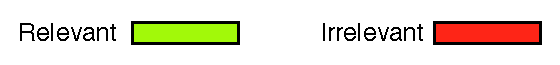
\includegraphics[width=5cm]{img/legend} 
\par\end{centering}

\begin{centering}
\subfigure[Title query.]{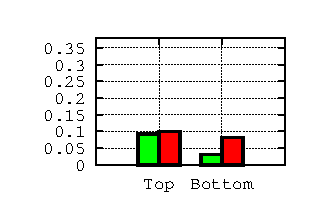
\includegraphics[width=4cm]{Results-CIKM2014/jaccard-qTitle-CLEF-IP2010}}\subfigure[Abstract query.]{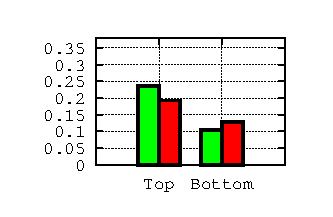
\includegraphics[width=4cm]{Results-CIKM2014/jaccard-qAbstract-CLEF-IP2010}} 
\par\end{centering}

\begin{centering}
\subfigure[Claims query.]{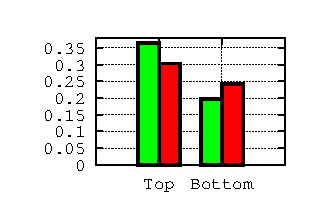
\includegraphics[width=4cm]{Results-CIKM2014/jaccard-qClaims-CLEF-IP2010}}\subfigure[Description query.]{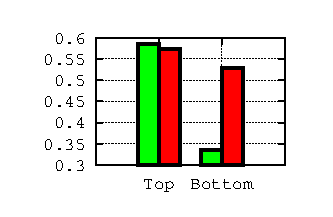
\includegraphics[width=4cm]{Results-CIKM2014/jaccard-qDescription-CLEF-IP2010}}
\caption{Average Jaccard similarity of (ir)relevant documents with the result
sets for different queries. }

\par\end{centering}

{\footnotesize{}{}%different queries (representing the title, abstract, or claims of a patent application)
%and the labeled (ir)relevant documents for the best (top) and worst (bottom) performing
%queries from CLEF-IP 2010 w.r.t. MAP.}
\label{fig:FailureAnalysis}} 
\end{figure}


While these results suggest the description section is the best part
of a partial patent application to use as query, they also point out
that the term overlap between the queries and the relevant documents
can be very low. Therefore, we suggest an investigation of \emph{query
reformulation} \cite{Baeza-Yates2010} methods as a means for improving
the term overlap between queries and relevant documents.

Query Reformulation is the process of transforming an initial query
$Q$ to another query $Q'$. This transformation may be either a reduction
or an expansion of the query. \emph{Query reduction} \cite{Kumaran2009}
reduces the query such that useless information is removed, while
\emph{query expansion} \cite{Efthimiadis1996} enhance the query with
additional terms likely to occur in relevant documents. In this paper,
we carry out an intensive study about query reformulation for patent
prior art search with partial patent applications, with the objective
of assessing not only the performance of standard query reformulation
methods, but also the effectiveness of query reformulation methods
that exploit patent-specific characteristics. In summary, the contributions
of this paper are the following: 
\begin{enumerate}
\item Novel contributions for query expansion and reduction that leverage
(a) patent structure and (b) term diversification techniques. 
\item A thorough comparative analysis of existing and novel methods for
query expansion and reduction in patent prior-art search on standardized
datasets of CLEF-IP. 
\end{enumerate}
The rest of this paper is organized as follows: in Section \ref{sec:QueryReformulationForPatents}
we present query reformulation frameworks; in Section \ref{sec:evaluation}
we present our evaluation framework and results analysis; and in Section
\ref{sec:conclusion} we conclude with possible directions for future
work.


\section{Query Reformulation for Patents}

\label{sec:QueryReformulationForPatents}

%In this section, we first present the requirements of a query expansion method in Sections \ref{sec:FrameworkQE}, then, we introduce a novel term selection method for query expansion in Section \ref{sec:MMRQE}. Next, in Section \ref{sec:FrameworkQR} we introduce the motivations behind the benefit of query reduction, and a new approach of query reduction in Section \ref{sec:MMRQR}.


During the exploration of query reformulation for patent search with
partial patent applications, there are many configuration options
and associated questions that we can consider: 
\begin{description}
\item [{Query type:}] We considered that a query of a partial patent application
consist of either the title, the abstract, the claims or the description
section. %\footnote{A query is always evaluated against the full content (title, abstract, claims, description) of granted patent applications since it is sensible to make use of all available content.}
Critical questions is: what part of a partial application an inventor
should write to obtain the best search results? %(ii) \textbf{what part of a patent application a patent examiner should use to make a patent prior art search? }

\item [{Relevance model:}] For initial retrieval of documents in the \emph{pseudo-relevant}
feedback set (PRF) %---\textbf{ often used to generate the terms for QE} ---
and subsequent re-retrieval, there are various options for the relevance
ranking model. In this work, we explore a probabilistic approach represented
by the popular BM25~\cite{Robertson1993} algorithm, as well as a
vector space model approach, TF-IDF~\cite{Salton1975}. A natural
question is which relevance model works best for query reformulation
for patent prior art search? 
\item [{Query expansion source:}] We can consider the title, abstract,
claims, and description sections as different term sources to determine
which section offers the best source of expansion terms, e.g., are
the title words of particularly high value as expansion terms? Note
that this only applies to query expansion methods. 
\item [{Term selection method:}] We consider different term selection
methods for query reformulation. We evaluate the performance of term
selection using Rocchio~\cite{Salton1971} and new term selection
methods that we propose in the next sections. %,which is intended to address the high-recall nature of patent prior art search. 
 Then a natural question is, which term selection method works best,
and with which configuration, i.e. query type, retrieval model, and
term source for query expansion methods? 
\end{description}
Before we proceed to evaluate the above questions, we first define
in Section \ref{sec:FrameworkQE} a novel term selection method for
QE hat we term MMRQE. This method is expected to address a potential
deficiency of Rocchio as used in practice for high-recall search.
Then, in Section \ref{sec:FrameworkQR} we present MMRQR, a novel
QR method, which is expected to rebuild the query from scratch by
selecting diversified terms.


\subsection{Query Expansion Frameworks (MMRQE)}

\label{sec:FrameworkQE}

As already mentioned, Query Expansion (QE)~\cite{Efthimiadis1996}
is a query reformulation approach that (automatically) adds terms
to an initial query in order to improve retrieval performance. The
utility of QE for patent prior art search is motivated by the term
overlap analysis depicted in Figure \ref{fig:FailureAnalysis}, which
illustrates that there is a large term mismatch between queries an
relevant documents. This term mismatch may be alleviated by QE methods.

% The following is a reasonable argument, but could be refuted by
% reviewers... term coverage and recall are more direct and simple
% arguments.


%Moreover, in contrast to scientific and technical writers, patent
%writers tend to generalize and maximize the scope of what is protected
%by a patent, and try to make sure that finding any relevant prior
%work by the patent examiner is a hard job. This leads to the usage
%of unusual expressions that makes finding similar patents a difficult
%task. This specificity of patents content led us to explore a method
%of term diversification selection for query expansion (the diversification
%here arise to select terms not only similar to the query to avoid
%the effect of its ambiguity). More specifically, we propose a new
%algorithm for query expansion based on the Maximal Marginal Relevance
%(MMR) \cite{Carbonell1998} method, which is an approach for result
%set diversification. We refer to our method from now on as MMRQE,
%which we define as a query expansion method that selects terms by
%carrying out a trade-off between diversification and similarity to
%the query.


As a term selection method in QE, Rocchio derives a score for each
potential query expansion term and in practice, the top-$k$ scoring
terms (often for $k\ll200$) are used to expand the query and are
weighted according to their Rocchio score during the second stage
of retrieval. The caveat of this approach is that given a limited
budget of $k$ expansion terms, there is no inherent guarantee that
these terms ``cover'' all documents in the pseudo-relevant set.
It seems that what we are asking for then is a method of ``diverse''
term selection --- such as the \emph{Maximal Marginal Relevance} (MMR)~\cite{Carbonell1998}
algorithm for result set diversification. But rather than use MMR
for diverse document selection (as typically used), we intend to use
it here for diverse term selection. In what follows, we present a
novel term selection method inspired by MMR, to address the deficiency
of Rocchio, that we call MMR Query Expansion (MMRQE).

%\subsubsection{MMR Query Expansion (MMRQE)}
%\label{sec:MMRQE}


%%%%%%%%%%%%%%%%%%%%%%%%%%%%%%%%%%%%%%%%%%%%%%%%%%%%%%%%%%%%%%%%%%%%%
\begin{figure}[t!]
\begin{centering}
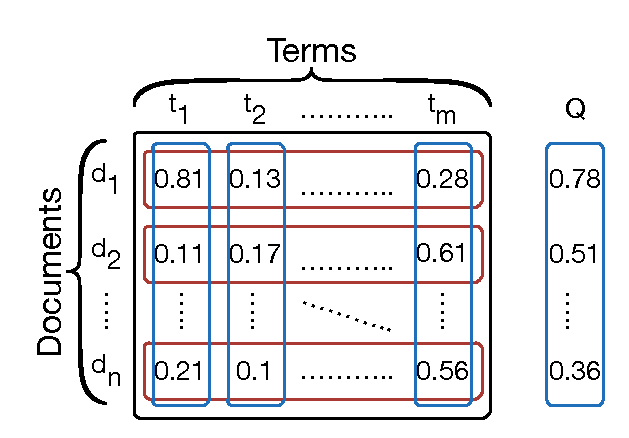
\includegraphics[width=5.5cm]{img/matrix} 
\par\end{centering}

\vspace{-1mm}
 \caption{Notation used in MMR QE/QR.}


\label{fig:notation} 
\end{figure}


%%%%%%%%%%%%%%%%%%%%%%%%%%%%%%%%%%%%%%%%%%%%%%%%%%%%%%%%%%%%%%%%%%%%%


We begin our formal description of MMRQE by first defining some necessary
notation. MMRQE takes as input a pseudo-relevant feedback set of $n$
documents (PRF), which is obtained after a retrieval for the initial
query. From the PRF set, we build a document-term matrix of $n$ documents
and $m$ terms as shown in Figure~\ref{fig:notation}, which uses
a TF-IDF weighting for each document vector (row $d_{i}$ for $1\leq i\leq n$).
However, as we will see shortly, the view that will be important for
us in this work is instead the term vector (column $t_{j}$ for $1\leq j\leq m$).
To represent the query $Q$ column vector in Figure~\ref{fig:notation}
having a numerical entry for every document $d_{i}$, we found that
computing the BM25 or TF-IDF score between each document $d_{i}$
and the query provided the best performance (in our experiments, the
score used is given by the indicated relevance model).

Given a query representation $Q$, we aim to select an optimal subset
of $k$ terms $T_{k}^{*}\subset D$ (where $|T_{k}^{*}|=k$ and $k\ll|m|$)
relevant to $Q$ but inherently different from each other (i.e., diverse).
This can be achieved by building $T_{k}^{*}$ in a greedy manner by
choosing the next optimal term $t_{k}^{*}$ given the previous set
of optimal term selections $T_{k-1}^{*}=\{t_{1}^{*},\ldots,t_{k-1}^{*}\}$
(assuming $T_{0}^{*}=\emptyset$) using the MMR diverse selection
criterion:

\begin{equation}
t_{k}^{*}=\argmax_{t_{k}\notin T_{k-1}^{*}}\hspace{-0.3mm}[\lambda\cos(Q,t_{k})-\hspace{-0.3mm}(1-\lambda)\max_{t_{j}\in T_{k-1}^{*}}\cos(t_{j},t_{k})]\label{eq:MMRQE-QR}
\end{equation}


Here, the first cosine similarity term measures relevance between
the query $Q$ and possible expansion term $t_{k}$ while the second
term penalizes the possible expansion term according to it's cosine
similarity with any currently selected term in $T_{k-1}^{*}$. The
parameter $\lambda\in[0,1]$ trades off relevance and diversity and
we found $\lambda=0.5$ to generally provide the best results in our
experiments on the CLEF-IP training dataset collection.

The key insight we want to conclude this section with is that MMRQE
does not select expansion terms independently as in practical usage
of Rocchio, but rather it selects terms that have uncorrelated usage
patterns across documents, thus hopefully encouraging diverse term
selection that covers more documents for a fixed expansion budget
$k$ and ideally, higher recall.


\subsection{Query Reduction Frameworks (MMRQR)}

\label{sec:FrameworkQR} 

As mentioned earlier, Query Reduction (QR)~\cite{Kumaran2009} is
a query reformulation method that attempts to reduce the query such
that superfluous information is removed. % NOTE: the sentence following this gets more to the point
%The patent sections: title,
%abstract, claims and description are of progressively increasing
%length. 
While the title is usually composed by an average of six terms, the
other sections are longer, ranging from ten to thousands of terms.
Therefore, we investigate the impact of query reduction methods when
querying with long sections such as abstract, claims and description.

Table \ref{tbl:queryPAC-1019} provides insight into the utility of
query reduction for the abstract section of the Topic PAC-1019 from
the CLEF-IP 2010 data collection. The baseline query, which is the
original query (provided in the header row) after stemming and patent
specific stopword removal, had an average precision (AP) of 0.280
and a patent retrieval evaluation score (PRES) \cite{Magdy2010a}
of 0.777 (its performance are provided in the footer row). We show
the evaluation performance of the query after removing each term from
the original query. The removed terms have been sorted in the order
of decreasing PRES. We can observe that there are ten terms (highlighted
in boldface) that if they are (individually) removed from the query,
we increase PRES of the original long query.

\begin{table}[h]
\begin{centering}
\caption{Sample of terms removed from the abstract section of CLEP-IP2010 Topic
PAC-1019. }

\par\end{centering}

\begin{centering}
{\footnotesize{}\label{tbl:queryPAC-1019}}
\par\end{centering}{\footnotesize \par}

\centering{}{\scriptsize{}}%
\begin{tabular}{|l|c|c|c|c|c|}
\hline 
\multicolumn{6}{|>{\raggedright}p{8cm}|}{\textbf{\scriptsize{}Topic:}{\scriptsize{} PAC-1019}}\tabularnewline
\hline 
\multicolumn{6}{|>{\raggedright}p{8cm}|}{\textbf{\scriptsize{}Abstract:}{\scriptsize{} A 5-aminolevulinic acid
salt which is useful in fields of microorganisms, fermentation, animals,
medicaments, plants and the like; a process for producing the same;
a medical composition comprising the same; and a plant activator composition
comprising the same.}}\tabularnewline
\hline 
\hline 
\textbf{\scriptsize{}Term removed} & \textbf{\scriptsize{}P@5} & \textbf{\scriptsize{}P@10} & \textbf{\scriptsize{}R@10} & \textbf{\scriptsize{}AP} & \textbf{\scriptsize{}PRES}\tabularnewline
\hline 
{\scriptsize{}composit...} & \textbf{\scriptsize{}0.600} & {\scriptsize{}0.300} & {\scriptsize{}0.428} & \textbf{\scriptsize{}0.360} & \textbf{\scriptsize{}0.829}\tabularnewline
\hline 
{\scriptsize{}activ...} & {\scriptsize{}0.400} & {\scriptsize{}0.300} & {\scriptsize{}0.428} & {\scriptsize{}0.277} & \textbf{\scriptsize{}0.809}\tabularnewline
\hline 
{\scriptsize{}anim...} & \textbf{\scriptsize{}0.600} & {\scriptsize{}0.300} & {\scriptsize{}0.428} & \textbf{\scriptsize{}0.345} & \textbf{\scriptsize{}0.798}\tabularnewline
\hline 
{\scriptsize{}produc...} & {\scriptsize{}0.400} & {\scriptsize{}0.300} & {\scriptsize{}0.428} & \textbf{\scriptsize{}0.286} & \textbf{\scriptsize{}0.797}\tabularnewline
\hline 
{\scriptsize{}ferment...} & {\scriptsize{}0.200} & {\scriptsize{}0.300} & {\scriptsize{}0.428} & \textbf{\scriptsize{}0.283} & \textbf{\scriptsize{}0.796}\tabularnewline
\hline 
{\scriptsize{}microorgan...} & \textbf{\scriptsize{}0.600} & {\scriptsize{}0.300} & {\scriptsize{}0.428} & \textbf{\scriptsize{}0.333} & \textbf{\scriptsize{}0.793}\tabularnewline
\hline 
{\scriptsize{}compris...} & {\scriptsize{}0.400} & {\scriptsize{}0.300} & {\scriptsize{}0.428} & {\scriptsize{}0.271} & \textbf{\scriptsize{}0.790}\tabularnewline
\hline 
{\scriptsize{}medica...} & {\scriptsize{}0.400} & {\scriptsize{}0.300} & {\scriptsize{}0.428} & \textbf{\scriptsize{}0.297} & \textbf{\scriptsize{}0.789}\tabularnewline
\hline 
{\scriptsize{}medic...} & {\scriptsize{}0.400} & {\scriptsize{}0.300} & {\scriptsize{}0.428} & \textbf{\scriptsize{}0.297} & \textbf{\scriptsize{}0.787}\tabularnewline
\hline 
{\scriptsize{}field...} & {\scriptsize{}0.400} & {\scriptsize{}0.300} & {\scriptsize{}0.428} & \textbf{\scriptsize{}0.282} & \textbf{\scriptsize{}0.782}\tabularnewline
\hline 
{\scriptsize{}plant...} & {\scriptsize{}0.200} & {\scriptsize{}0.200} & {\scriptsize{}0.285} & {\scriptsize{}0.114} & {\scriptsize{}0.774}\tabularnewline
\hline 
{\scriptsize{}process...} & {\scriptsize{}0.400} & {\scriptsize{}0.300} & {\scriptsize{}0.428} & {\scriptsize{}0.279} & {\scriptsize{}0.764}\tabularnewline
\hline 
{\scriptsize{}acid...} & {\scriptsize{}0.400} & {\scriptsize{}0.300} & {\scriptsize{}0.428} & {\scriptsize{}0.252} & {\scriptsize{}0.693}\tabularnewline
\hline 
{\scriptsize{}salt...} & {\scriptsize{}0.200} & {\scriptsize{}0.200} & {\scriptsize{}0.285} & {\scriptsize{}0.216} & {\scriptsize{}0.663}\tabularnewline
\hline 
{\scriptsize{}aminolevulin...} & {\scriptsize{}0.000} & {\scriptsize{}0.100} & {\scriptsize{}0.142} & {\scriptsize{}0.026} & {\scriptsize{}0.352}\tabularnewline
\hline 
\hline 
\textbf{\scriptsize{}Baseline} & {\scriptsize{}0.400} & {\scriptsize{}0.300} & {\scriptsize{}0.428} & {\scriptsize{}0.280} & {\scriptsize{}0.777}\tabularnewline
\hline 
\end{tabular}
\end{table}


Figure \ref{fig:QRUtility} shows the summary upper-bound performance
for precision, recall, MAP, Mean Reciprocal Rank (MRR), and PRES that
can be achieved for a set of 1304 abstract queries from the CLEF-IP
2010 data collection. ``Baseline\textquotedblright{} refers to a
probabilistic BM25 retrieval model ~\cite{Robertson1993} run using
the Lucene search engine \cite{McCandless2010} and the original long
query. ``Oracle\textquotedblright{} refers to the situation where
all terms with negative impact are removed from the original long
query following the previous process. This gives us an upper bound
on the performance that can be realized through query reduction for
this set of queries. It is this statistically significant improvement
in performance through query reduction that we target in this second
part of our work for all query sections, i.e. title, abstract, claims,
and description.

\begin{figure}[!h]
\begin{centering}
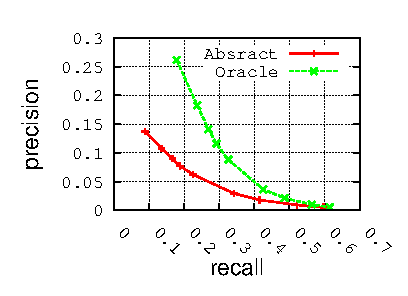
\includegraphics[width=4cm]{analysis/precision-recall_ByField-CLEF-IP_2010}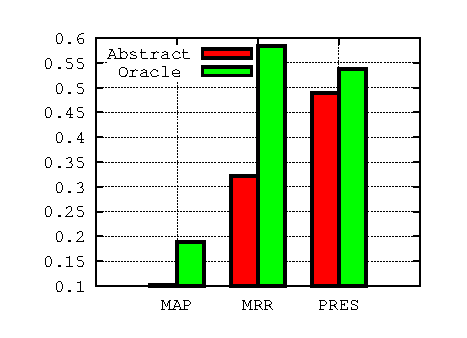
\includegraphics[width=4cm]{analysis/MAP-MRR_ByField-CLEF-IP_2010}
\caption{The utility of query reduction for 1304 abstract queries of the CLEF-IP
2010 dataset. }

\par\end{centering}

\begin{centering}
{\footnotesize{}\label{fig:QRUtility}}
\par\end{centering}{\footnotesize \par}

{\footnotesize{}%different queries (representing the title, abstract, or claims of a patent application)
%and the labeled (ir)relevant documents for the best (top) and worst (bottom) performing
%queries from CLEF-IP 2010 w.r.t. MAP.}
}
\end{figure}


Following the same motivations than those which led us to propose
MMRQR, we propose to greedily rebuild the query from its terms, while
choosing diversified terms. Formally, given a query representation
$Q$, we aim to select an optimal subset of $k$ terms $T_{k}^{*}\subset Q$
(where $|T_{k}^{*}|=k$ and $k<|Q|$) relevant to $Q$ but inherently
different from each other (i.e., diverse). This can be achieved by
building $T_{k}^{*}$ in a greedy manner by choosing the next optimal
term $t_{k}^{*}$ given the previous set of optimal term selections
$T_{k-1}^{*}=\{t_{1}^{*},\ldots,t_{k-1}^{*}\}$ (assuming $T_{0}^{*}=\emptyset$)
using an adaptation of the MMR diverse selection criterion as given
in Equation \ref{eq:MMRQE-QR}. Note that the we used all the sections
of the patent documents of the PRF set to built the document-term
matrix of $n$ documents and $m$ terms shown in Figure~\ref{fig:notation}.
Here, we found that $\lambda=0.8$ provides generally the best results
in our experiments on the CLEF-IP training dataset collection.

In the next section, we propose a deep evaluation of QE and QR methods
for patent search, and we attempt to answer the questions we asked
in the beginning of this section.


\section{Experimental Evaluation}

\label{sec:evaluation}

In this section we first explain our experimental setup for evaluating
the effectiveness of the different methods. Then, we discuss the results
of QE and QR methods.


\subsection{Experimental Setup}

We used the Lucene IR System%
\footnote{We used the LucQE module, which provides an implementation of the
Rocchio QE method for Lucene. \\ \texttt{http://lucene-qe.sourceforge.net/}%
} to index the English subset of CLEF-IP 2010 and CLEF-IP 2010 datasets%
\footnote{\texttt{\url{http://www.ifs.tuwien.ac.at/~clef-ip/}}%
}~\cite{Piroi2011,Roda2009} with the default stemming and stop-word
removal. We removed patent-specific stop-words as described in \cite{Magdy2012}.
CLEF-IP 2010 contains 2.6 million patent documents and CLEF-IP 2011
consists of 3 million patent documents. The English test sets of CLEF-IP
2010 and CLEF-IP 2011 correspond to 1303 and 1351 topics respectively.
In our implementation, each section of a patent (title, abstract,
claims, and description) is indexed in a separate field, so that different
sections can be used, for example, as source of expansion terms. But,
when a query is processed, all fields in the index are targeted, since
it is sensible to use all available content.

We also used the patent classification (IPC) for filtering the results
by constraining them to have common classifications with the patent
topic as suggested in previous works \cite{Lopez2009,Roda2009}. Finally,
we report Mean Average Precision (MAP), and Patent Retrieval Evaluation
Score (PRES) \cite{Magdy2010a}, which combines Recall with the quality
of ranking and weights relevant documents lower in the ranking more
highly than MAP. We report the evaluation metrics on the top 1000
results.

%\begin{figure}
%\begin{centering}
%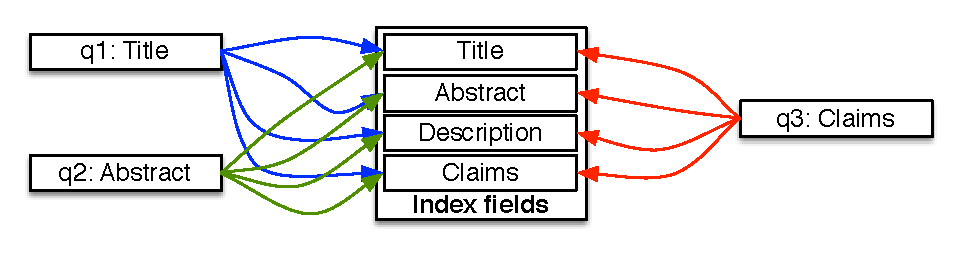
\includegraphics[width=8cm]{img/matching}
%\par\end{centering}
%\caption{Model of the index fields matching with queries .}
%\label{fig:IndexFields}
%\end{figure}



\subsection{Experimental Results for QE}


\subsubsection{Query Expansion Baselines}

In addition to the general Rocchio approach for QE, we included two
other patent specific QE methods as baselines. Motivated by \cite{Mahdabi2013},
we used the text definitions of the International Patent Classification
(IPC) codes assigned to a patent application as a source for query
expansion --- this is denoted as \textbf{IPC Codes}. We also implemented
the QE approach proposed in \cite{Magdy2011}, which automatically
generates candidate synonyms sets (SynSet) for terms, and use it as
a source of expansion terms. This approach has two variants: (i) The
first one use the probability associated with the SynSet entries as
a weight for each expanded term in the query (denoted \textbf{WSynSet}).
Therefore, each term was replaced with its SynSet entries with the
probability of each item in the SynSet acting as a weight to the term
within the query. (ii) The second one neglected this associated probability
and used uniform weighting for all synonyms of a given term (denoted
\textbf{USynSet}). The combination of QE methods, relevance model
and term selection options give us seven QE algorithms to evaluate.
When MMRQE is used in combination with the VSM, the additional terms
use the weights provided by the Rocchio method, whereas when using
MMRQE and Rocchio with BM25, there is no need to weight the terms.
For all methods, their parameters were fixed to their optimal values,
which were estimated using the CLEF-IP training queries.

Other QE methods have been also explored for patent prior art search.
For example, Magdy et al. \cite{Magdy2011} experiment a set of classic
techniques of query expansion, which rely WordNet as source of expansion
terms. However, none of these approaches were able to achieve a significant
improvement over the baseline/queries without expansion. Also, Bashir
et al. \cite{Bashir2010} propose a query expansion with pseudo-relevance
feedback. They proposed to select relevant terms for the expansion
process using a machine learning approach, by picking terms that may
have a potential positive impact on the retrieval effectiveness. However,
this approach can be computational expensive, since the presented
features are complicated to compute. Verma and Varma \cite{Verma2011}
propose a different approach, which instead of using the patent text
to query, they use its International Patent Classification (IPC) codes
as query which are expanded using the citation network. The formed
query is used to perform an initial search. The results are then re-ranked
using queries constructed from patent text. Throughout our experiments,
we concluded that relying on other terms to form a query rather than
those in the patent application, leads to poor retrieval quality.
Therefore, the approach proposed in \cite{Verma2011} doesn't guarantee
to obtain good performance. %
\begin{comment}
Lastly, a more recent work by Mahdabi et al. \cite{Mahdabi2013} propose
a query expansion method that build a query-specific patent lexicon
based on the definitions of the IPC. Then, this patent lexicon is
used to select expansion terms that are focused on the query topic.
\end{comment}



\subsubsection{Discussion}

In this section, we discuss the results of the evaluation performed
on the QE methods described above. But before, we first discuss the
effect of the size of the PRF set on the performance. Table \ref{tbl:PFRSize}
shows the impact of the PRF size on the performance for the two QE
algorithms Rocchio and MMRQE. These results are shown on the CLEF-IP
2010 training dataset, which consists of 196 topics. We observe that
the best QE performance results are obtained when using few documents
in the PRF set as it was also reported in \cite{Magdy2011} (in our
case, the top five gave the best results). This is certainly due to
the fact that a large PRF set will include too much irrelevant documents,
whose the terms may negatively affect the quality of the expanded
query.

\begin{table}[h]
\caption{Effect of PRF with various numbers of feedback documents on the CLEF-IP
2010 dataset. 20 terms are used for query expansion.}
\label{tbl:PFRSize}

\centering{}{\scriptsize{}}%
\begin{tabular}{|l|c|c|c|c|c|}
\hline 
\textbf{\scriptsize{}Query/Source} & \textbf{\scriptsize{}Metric} & \textbf{\scriptsize{}Method} & \textbf{\scriptsize{}5} & \textbf{\scriptsize{}10} & \textbf{\scriptsize{}20}\tabularnewline
\hline 
\hline 
{\scriptsize{}Query: Abstract} & {\scriptsize{}MAP} & {\scriptsize{}Rocchio} & {\scriptsize{}0.074} & {\scriptsize{}0.072} & {\scriptsize{}0.070}\tabularnewline
\cline{3-6} 
 & {\scriptsize{}BL=0.073} & {\scriptsize{}MMRQE} & {\scriptsize{}0.074} & {\scriptsize{}0.071} & {\scriptsize{}0.071}\tabularnewline
\cline{2-6} 
{\scriptsize{}Source: Claims} & {\scriptsize{}PRES} & {\scriptsize{}Rocchio} & {\scriptsize{}0.409} & {\scriptsize{}0.409} & {\scriptsize{}0.409}\tabularnewline
\cline{3-6} 
 & \multirow{1}{*}{{\scriptsize{}BL=0.403}} & {\scriptsize{}MMRQE} & {\scriptsize{}0.411} & {\scriptsize{}0.411} & {\scriptsize{}0.410}\tabularnewline
\hline 
{\scriptsize{}Query: Claims} & {\scriptsize{}MAP} & {\scriptsize{}Rocchio} & {\scriptsize{}0.083} & {\scriptsize{}0.080} & {\scriptsize{}0.079}\tabularnewline
\cline{3-6} 
 & {\scriptsize{}BL=0.081} & {\scriptsize{}MMRQE} & {\scriptsize{}0.082} & {\scriptsize{}0.080} & {\scriptsize{}0.080}\tabularnewline
\cline{2-6} 
{\scriptsize{}Source: Claims} & {\scriptsize{}PRES} & {\scriptsize{}Rocchio} & {\scriptsize{}0.443} & {\scriptsize{}0.445} & {\scriptsize{}0.446}\tabularnewline
\cline{3-6} 
 & {\scriptsize{}BL=0.433} & {\scriptsize{}MMRQE} & {\scriptsize{}0.445} & {\scriptsize{}0.444} & {\scriptsize{}0.442}\tabularnewline
\hline 
\end{tabular}
\end{table}


\begin{comment}
As recommended in \cite{Magdy2012} and confirmed in our own experimentation
(not shown due to lack of space), best QE performance results are
obtained when using few documents in the PRF set (in our case, the
top five gave the best results).
\end{comment}
{} 

Next, we carry out comprehensive experiments along the dimensions
outlined in Section~\ref{sec:FrameworkQE} with the following specific
options:
\begin{itemize}
\item \textbf{\footnotesize{}Query type:}{\footnotesize{} $\{\mathrm{Title},\mathrm{Abstract},\mathrm{Claims},\mathrm{Description}\}$ }{\footnotesize \par}
\item \textbf{\footnotesize{}Query expansion source:}{\footnotesize{} $\{\mathrm{Title},\mathrm{Abs.},\mathrm{Claims},\mathrm{Descrip.}\}$ }{\footnotesize \par}
\item \textbf{\footnotesize{}Relevance model:}{\footnotesize{} $\{\mathrm{BM25},\mbox{Vector-space Model (VSM)}\}$ }{\footnotesize \par}
\item \textbf{\footnotesize{}Term selection method:}{\footnotesize{} $\{\mathrm{Rocchio},\mathrm{MMRQE},etc...\}$ }{\footnotesize \par}
\end{itemize}
Figure \ref{fig:QE-qClaims-sAbstract-CLEF-2010} shows the results
obtained in terms of MAP and PRES for CLEF-IP 2010 for different numbers
of expanded terms $k$ on the x-axis (with $k=0$ using no QE, just
the baseline retrieval model). For lack of space we show only the
results of queries extracted from the claims and the abstract used
as source of query expansion. From these results, we make the following
observations: (i) for the two retrieval models (VSM and BM25), MMRQE
provides the best performance for both MAP and PRES (except for MAP,
where Rocchio BM25 provides better performance than MMRQE BM25), (ii)
for both MMRQE and Rocchio, the best performance is obtained while
adding no more than 50 terms to the original queries (adding more
terms may have no effect, or decrease the performance), and (iii)
exploiting external sources for query expansion provides poor performance
(IPC code definition and SynSets). 

\begin{center}
\begin{figure}[h]
\begin{centering}
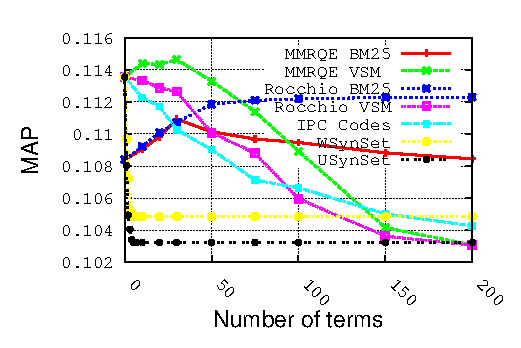
\includegraphics[width=4.3cm]{Results-CIKM2014/qClaims-sAbstract_MAP_2010}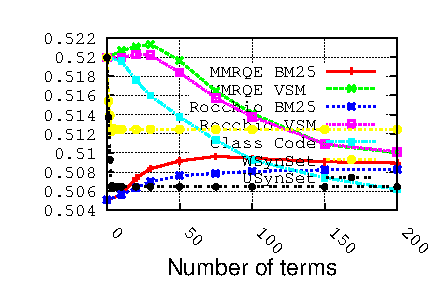
\includegraphics[width=4.3cm]{Results-CIKM2014/qClaims-sAbstract_PRES_2010}
\par\end{centering}

\caption{Results obtained while using the claims for querying and the abstract
as source of query expansion on the CLEF-IP 2010.}


\label{fig:QE-qClaims-sAbstract-CLEF-2010}
\end{figure}

\par\end{center}

To summarize all the results obtained over all the above configurations,
Figures~\ref{fig:MAP-CLEF2010}, ~\ref{fig:PRES-CLEF2010},~\ref{fig:MAP-CLEF2011},
and~\ref{fig:PRES-CLEF2011} show the performance obtained for all
the QE methods, while selecting the optimal number of terms used for
the expansion (number of terms that maximizes the performance for
each method). From these results, we first observe that the best section
to use for querying is the description section (see Figures \ref{fig:qDescription-MAP-CLEF-IP2010},
\ref{fig:qDescription-PRES-CLEF-IP2010}, \ref{fig:qDescription-MAP-CLEF-IP2011},
and \ref{fig:qDescription-PRES-CLEF-IP2011}). We attribute this to
the fact that the description section has more content along with
more terms relevant to specific details that describe the patent,
since the core of the invention is described therein.

Secondly, regarding the source of query expansion, we observe that
the best source is the claims. We attribute this to the fact that
the claims section has more technical terms, which may be common with
relevant patents, since legal aspects of the invention are described
therein. However, when querying using the claims, other sources of
query expansion may provide better performance. This may be because
the query needs more general terms than the technical/legal terms
already in the claims section. It is interesting to notice that the
description is not either a good source for expansion, since it may
contain more general terms that may hurt the performance.

Thirdly, we observed that query expansion is not useful for very long
queries (i.e. description), indicating that in advanced stages of
the patent application process, QE is not relevant. We also notice
that when dealing with more complex queries such as abstract or claims,
MMRQE is more effective than Rocchio, which suggest that diverse term
selection is not crucial for short queries.

Finally, we observed that using the IPC code definitions (as suggested
by \cite{Mahdabi2013}) and SynSet (method of \cite{Magdy2011}) as
a source of expansion, gave poor performance (see IPC Codes and SynSet
bars along the Figures).

%\begin{figure*}[t]
%\begin{centering}
%\subfigure[{\tiny Query Claims \& source Title.}]{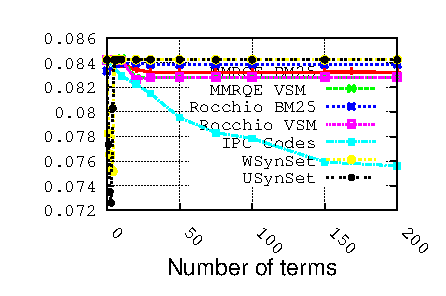
\includegraphics[width=4.3cm]{Results-SIGIR2014/qClaims-sTitle_MAP_2011}}\subfigure[{\tiny Query Claims \& source Abstract.}]{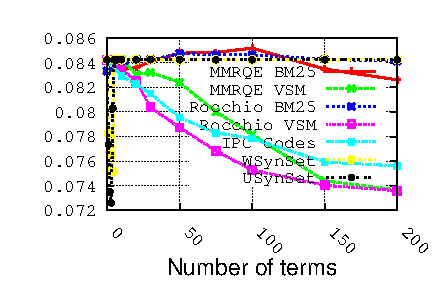
\includegraphics[width=4.3cm]{Results-SIGIR2014/qClaims-sAbstract_MAP_2011}}\subfigure[{\tiny Query Claims \& source Claims.}]{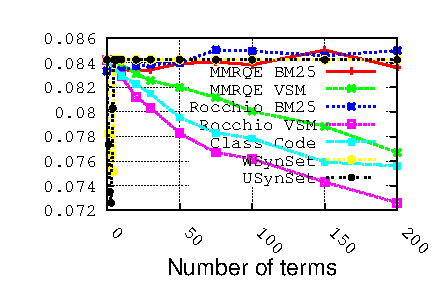
\includegraphics[width=4.3cm]{Results-SIGIR2014/qClaims-sClaims_MAP_2011}}\subfigure[{\tiny Query Claims \& source Descrip.}]{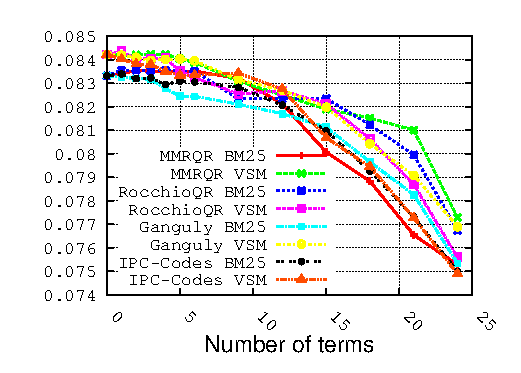
\includegraphics[width=4.3cm]{Results-SIGIR2014/qClaims-sDescription_MAP_2011}}
%\par\end{centering}
%\vspace{-3mm}
%\caption{Mean Average Precision (MAP) on CLEF-2011 (for MMRQE $\lambda=0.5$).}
%\label{fig:MAP-CLEF2011}
%\vspace{-3mm}
%\end{figure*}


%\begin{figure*}
%\begin{centering}
%\subfigure[{\tiny Query Claims \& source Title.}]{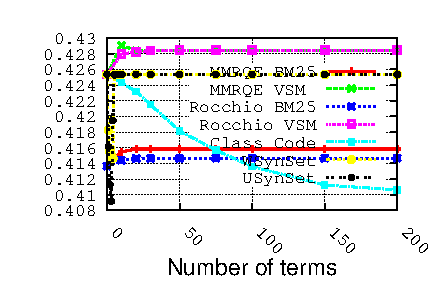
\includegraphics[width=4.3cm]{Results-SIGIR2014/qClaims-sTitle_PRES_2011}}\subfigure[{\tiny Query Claims \& source Abstract.}]{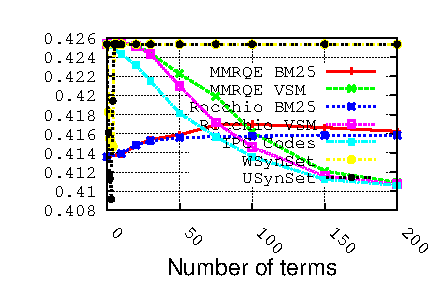
\includegraphics[width=4.3cm]{Results-SIGIR2014/qClaims-sAbstract_PRES_2011}}\subfigure[{\tiny Query Claims \& source Claims.}]{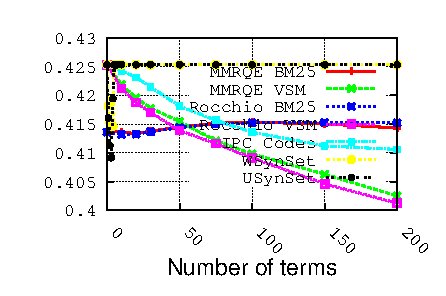
\includegraphics[width=4.3cm]{Results-SIGIR2014/qClaims-sClaims_PRES_2011}}\subfigure[{\tiny Query Claims \& source Descrip.}]{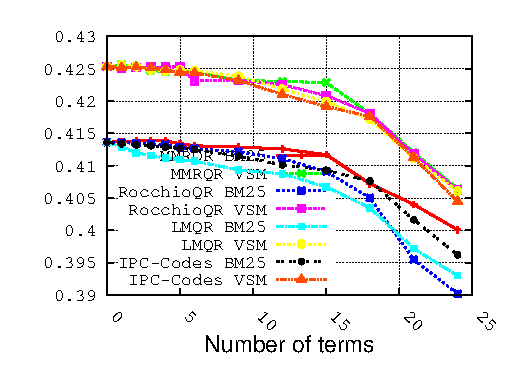
\includegraphics[width=4.3cm]{Results-SIGIR2014/qClaims-sDescription_PRES_2011}}
%\par\end{centering}
%\vspace{-3mm}
%\caption{Patent Retrieval Evaluation Score (PRES) on CLEF-2011 (for MMRQE $\lambda=0.5$).}
%\label{fig:PRES-CLEF2011}
%\vspace{-3mm}
%r\end{figure*}


Regarding the best term selection method, we conclude that in general
MMRQE provides better performance than Rocchio. To give an insight
of the effect of MMRQE and Rocchio over the performance, Table \ref{tbl:QESampleQueries}
shows some queries where QE methods improved the performance. First
of all, it is interesting to notice that even if there are common
terms selected to expand the queries by both MMRQE and Rocchio, the
lists of MMRQE contain more diversified terms (at least in the two
first examples). For the two first examples, relevant patents talk
about a similar idea than the applications, but using different examples
and applications (the writers of a patent use complex and ambiguous
terms to generalize the coverage of the invention). Hence, for the
first query, key terms like: \textit{rotor, blend, and suction}, were
able to capture the scope of the relevant patents to allow either
retrieving them (improving PRES), or pushing them to the top of the
ranking (improving MAP). As for the third query, MMRQE expand the
query with general terms, e.g. \textit{result, includ, extend, plural},
which probably encourage retrieving irrelevant patents.

\begin{table*}[t]
\caption{Samples of queries extracted from CLEF-IP 2011, where QE improves
the performance (P: Precision, R: Recall, RR: Reciprocal Rank, AP:
Average Precision, PRES: Patent Retrieval Evaluation Score). MMRQE
improves the two first examples, while Rocchio improves the third. }
\label{tbl:QESampleQueries}

\centering{}%
\begin{tabular}{|>{\raggedright}p{17.5cm}|}
\hline 
\textbf{\scriptsize{}1- Topic:}{\scriptsize{} EP-1921264-A2}\tabularnewline
\hline 
\textbf{\scriptsize{}Abstract:}{\scriptsize{} An article of manufacture
having a nominal profile substantially in accordance with Cartesian
coordinate values of X, Y and Z set forth in a TABLE 1. Wherein X
and Y are distances in inches which, when connected by smooth continuing
arcs, define airfoil profile sections at each distance Z in inches.
The profile sections at the Z distances being joined smoothly with
one another to form a complete airfoil shape (22,23).}\tabularnewline
\hline 
\begin{tabular}{>{\centering}p{16.5cm}}
{\scriptsize{}Baseline performance:}~{\scriptsize{}}%
\begin{tabular}{|c|c|c|c|c|c|c|c|c|c|c|c|}
\hline 
\textbf{\scriptsize{}P@5:} & {\scriptsize{}0.000} & \textbf{\scriptsize{}P@10:} & {\scriptsize{}0.000} & \textbf{\scriptsize{}R@10:} & {\scriptsize{}0.000} & \textbf{\scriptsize{}RR:} & {\scriptsize{}0.066} & \textbf{\scriptsize{}AP:} & {\scriptsize{}0.043} & \textbf{\scriptsize{}PRES:} & {\scriptsize{}0.777}\tabularnewline
\hline 
\end{tabular}\tabularnewline
\end{tabular}\tabularnewline
\hline 
\textbf{\scriptsize{}MMRQE expanded terms:}{\scriptsize{} }\textbf{\scriptsize{}\uline{airfoil}}{\scriptsize{},
}\textbf{\scriptsize{}rotor}{\scriptsize{}, }\textbf{\scriptsize{}blend}{\scriptsize{},
}\textbf{\scriptsize{}substanti}{\scriptsize{}, }\textbf{\scriptsize{}\uline{root}}{\scriptsize{},
}\textbf{\scriptsize{}\uline{portion}}{\scriptsize{}, }\textbf{\scriptsize{}includ}{\scriptsize{},
}\textbf{\scriptsize{}suction}{\scriptsize{}, }\textbf{\scriptsize{}\uline{form}}{\scriptsize{},
}\textbf{\scriptsize{}tip}\tabularnewline
\hline 
\begin{tabular}{>{\centering}p{16.5cm}}
{\scriptsize{}MMRQE performance:}~{\scriptsize{}}%
\begin{tabular}{|c|c|c|c|c|c|c|c|c|c|c|c|}
\hline 
\textbf{\scriptsize{}P@5:} & {\scriptsize{}0.000} & \textbf{\scriptsize{}P@10:} & {\scriptsize{}0.200} & \textbf{\scriptsize{}R@10:} & {\scriptsize{}0.666} & \textbf{\scriptsize{}RR:} & {\scriptsize{}0.142} & \textbf{\scriptsize{}AP:} & {\scriptsize{}0.124} & \textbf{\scriptsize{}PRES:} & {\scriptsize{}0.872}\tabularnewline
\hline 
\end{tabular}\tabularnewline
\end{tabular}\tabularnewline
\hline 
\textbf{\scriptsize{}Rocchio expanded terms:}\textit{\scriptsize{}
}\textbf{\scriptsize{}\uline{airfoil}}{\scriptsize{}, }{\scriptsize{}\uline{trail}}{\scriptsize{},
}{\scriptsize{}\uline{edg}}{\scriptsize{}, }{\scriptsize{}\uline{cool}}{\scriptsize{},
}\textbf{\scriptsize{}\uline{form}}{\scriptsize{}, }{\scriptsize{}\uline{blade}}{\scriptsize{},
}{\scriptsize{}\uline{side}}{\scriptsize{}, }\textbf{\scriptsize{}\uline{portion}}{\scriptsize{},
}\textbf{\scriptsize{}\uline{root}}{\scriptsize{}, }{\scriptsize{}\uline{lead}}\tabularnewline
\hline 
\begin{tabular}{>{\centering}p{16.5cm}}
{\scriptsize{}Rocchio performance:}~{\scriptsize{}}%
\begin{tabular}{|c|c|c|c|c|c|c|c|c|c|c|c|}
\hline 
\textbf{\scriptsize{}P@5:} & {\scriptsize{}0.000} & \textbf{\scriptsize{}P@10:} & {\scriptsize{}0.100} & \textbf{\scriptsize{}R@10:} & {\scriptsize{}0.333} & \textbf{\scriptsize{}RR:} & {\scriptsize{}0.142} & \textbf{\scriptsize{}AP:} & {\scriptsize{}0.100} & \textbf{\scriptsize{}PRES:} & {\scriptsize{}0.822}\tabularnewline
\hline 
\end{tabular}\tabularnewline
\end{tabular}\tabularnewline
\hline 
\hline 
\textbf{\scriptsize{}2- Topic: }{\scriptsize{}EP-1707587-A1}\tabularnewline
\hline 
\textbf{\scriptsize{}Abstract:}{\scriptsize{} It is intended to provide
a crosslinked polyrotaxane formed by crosslinking polyrotaxane moleculesvia
chemical bonds which exhibits excellent optical properties in water
or in an aqueous solution of sodium chloride; a compound having this
crosslinked polyrotaxane; and a process for producing the same. The
above object can be achieved by a crosslinked polyrotaxane having
at least two polyrotaxane molecules, wherein linear molecules are
included in a skewered-like state at the opening of cyclodextrin molecules
and blocking groups are provided at both ends of the linear molecules,
so as to prevent the cyclodextrin molecules from leaving, and cyclodextrin
molecules in at least two polyrotaxane molecules being bonded to each
other via chemical bond, characterized in that hydroxyl (-OH) groups
in the cyclodextrin molecules are partly substituted with non-ionic
groups. }\tabularnewline
\hline 
\begin{tabular}{>{\centering}p{16.5cm}}
{\scriptsize{}Baseline performance:}~{\scriptsize{}}%
\begin{tabular}{|c|c|c|c|c|c|c|c|c|c|c|c|}
\hline 
\textbf{\scriptsize{}P@5:} & {\scriptsize{}0.400} & \textbf{\scriptsize{}P@10:} & {\scriptsize{}0.300} & \textbf{\scriptsize{}R@10:} & {\scriptsize{}0.600} & \textbf{\scriptsize{}RR:} & {\scriptsize{}1.000} & \textbf{\scriptsize{}AP:} & {\scriptsize{}0.477} & \textbf{\scriptsize{}PRES:} & {\scriptsize{}0.784}\tabularnewline
\hline 
\end{tabular}\tabularnewline
\end{tabular}\tabularnewline
\hline 
\textbf{\scriptsize{}MMRQE expanded terms: }\textbf{\scriptsize{}\uline{bond}}{\scriptsize{},
}\textbf{\scriptsize{}\uline{includ}}{\scriptsize{}, }\textbf{\scriptsize{}\uline{thereof}}{\scriptsize{},
}\textbf{\scriptsize{}convent}{\scriptsize{}, }\textbf{\scriptsize{}\uline{crosslink}}{\scriptsize{},
}\textbf{\scriptsize{}\uline{plural}}{\scriptsize{}, }\textbf{\scriptsize{}polyrotaxan}{\scriptsize{},
}\textbf{\scriptsize{}substanc}{\scriptsize{}, }\textbf{\scriptsize{}gelatin}{\scriptsize{},
}\textbf{\scriptsize{}fractur}{\scriptsize{}, }\textbf{\scriptsize{}realiz}{\scriptsize{},
}\textbf{\scriptsize{}uniform}{\scriptsize{}, }\textbf{\scriptsize{}chemic}{\scriptsize{},
}\textbf{\scriptsize{}physic}{\scriptsize{}, }\textbf{\scriptsize{}rotat}{\scriptsize{},
}\textbf{\scriptsize{}biodegrad}{\scriptsize{}, }\textbf{\scriptsize{}expans}{\scriptsize{},
}\textbf{\scriptsize{}resist}{\scriptsize{}, }\textbf{\scriptsize{}elast}{\scriptsize{},
}\textbf{\scriptsize{}entrop}\tabularnewline
\hline 
\begin{tabular}{>{\centering}p{16.5cm}}
{\scriptsize{}MMRQE performance:}~{\scriptsize{}}%
\begin{tabular}{|c|c|c|c|c|c|c|c|c|c|c|c|}
\hline 
\textbf{\scriptsize{}P@5:} & {\scriptsize{}0.600} & \textbf{\scriptsize{}P@10:} & {\scriptsize{}0.300} & \textbf{\scriptsize{}R@10:} & {\scriptsize{}0.600} & \textbf{\scriptsize{}RR:} & {\scriptsize{}1.000} & \textbf{\scriptsize{}AP:} & {\scriptsize{}0.577} & \textbf{\scriptsize{}PRES:} & {\scriptsize{}0.797}\tabularnewline
\hline 
\end{tabular}\tabularnewline
\end{tabular}\tabularnewline
\hline 
\textbf{\scriptsize{}Rocchio expanded terms: }{\scriptsize{}\uline{form}}{\scriptsize{},
}{\scriptsize{}\uline{present}}{\scriptsize{}, }{\scriptsize{}\uline{cyclodextrin}}{\scriptsize{},
}{\scriptsize{}\uline{compris}}{\scriptsize{}, }{\scriptsize{}\uline{molecul}}{\scriptsize{},
}{\scriptsize{}\uline{polym}}{\scriptsize{}, }\textbf{\scriptsize{}\uline{includ}}{\scriptsize{},
}\textbf{\scriptsize{}\uline{crosslink}}{\scriptsize{}, }{\scriptsize{}\uline{group}}{\scriptsize{},
}{\scriptsize{}\uline{compound}}{\scriptsize{}, }{\scriptsize{}\uline{relat}}{\scriptsize{},
}{\scriptsize{}\uline{contact}}{\scriptsize{}, }{\scriptsize{}\uline{water}}{\scriptsize{},
}{\scriptsize{}\uline{monom}}{\scriptsize{}, }{\scriptsize{}\uline{linear}}{\scriptsize{},
}{\scriptsize{}\uline{composit}}{\scriptsize{}, }\textbf{\scriptsize{}\uline{thereof}}{\scriptsize{},
}{\scriptsize{}\uline{materi}}{\scriptsize{}, }\textbf{\scriptsize{}\uline{plural}}{\scriptsize{},
}\textbf{\scriptsize{}\uline{bond}}\tabularnewline
\hline 
\begin{tabular}{>{\centering}p{16.5cm}}
{\scriptsize{}Rocchio performance:}~{\scriptsize{}}%
\begin{tabular}{|c|c|c|c|c|c|c|c|c|c|c|c|}
\hline 
\textbf{\scriptsize{}P@5:} & {\scriptsize{}0.400} & \textbf{\scriptsize{}P@10:} & {\scriptsize{}0.200} & \textbf{\scriptsize{}R@10:} & {\scriptsize{}0.400} & \textbf{\scriptsize{}RR:} & {\scriptsize{}1.000} & \textbf{\scriptsize{}AP:} & {\scriptsize{}0.455} & \textbf{\scriptsize{}PRES:} & {\scriptsize{}0.770}\tabularnewline
\hline 
\end{tabular}\tabularnewline
\end{tabular}\tabularnewline
\hline 
\hline 
\textbf{\scriptsize{}3- Topic: }{\scriptsize{}EP-1754935-A1}\tabularnewline
\hline 
\textbf{\scriptsize{}Abstract:}{\scriptsize{} The fire-rated recessed
downlight includes a mantle. A radiating mouth (4) is defined in the
mantle. A dilatable fireproof piece (5) is fixed in the radiating
mouth (4). Radiating apertures (6 or 6') corresponding to the radiating
mouth (4) is defined in the dilatable fireproof piece (5) or between
edges of the dilatable fireproof piece (5) and edges of the radiating
mouth (4). The radiating mouth (4) of the mantle and the dilatable
fireproof piece (5) could help to radiate the heat in ordinary situation
and the dilatable fireproof piece (5) will expand rapidly to close
the radiating mouth (4) when on fire, therefore the fire inside the
mantle will not spread to the outside.}\tabularnewline
\hline 
\begin{tabular}{>{\centering}p{16.5cm}}
{\scriptsize{}Baseline performance:}~{\scriptsize{}}%
\begin{tabular}{|c|c|c|c|c|c|c|c|c|c|c|c|}
\hline 
\textbf{\scriptsize{}P@5:} & {\scriptsize{}0.200} & \textbf{\scriptsize{}P@10:} & {\scriptsize{}0.100} & \textbf{\scriptsize{}R@10:} & {\scriptsize{}0.111} & \textbf{\scriptsize{}RR:} & {\scriptsize{}0.250} & \textbf{\scriptsize{}AP:} & {\scriptsize{}0.086} & \textbf{\scriptsize{}PRES:} & {\scriptsize{}0.801}\tabularnewline
\hline 
\end{tabular}\tabularnewline
\end{tabular}\tabularnewline
\hline 
\textbf{\scriptsize{}MMRQE expanded terms: }\textbf{\scriptsize{}\uline{mmateri}}{\scriptsize{},
}\textbf{\scriptsize{}\uline{adapt}}{\scriptsize{}, }\textbf{\scriptsize{}\uline{2}}{\scriptsize{},
}\textbf{\scriptsize{}\uline{hous}}{\scriptsize{}, }\textbf{\scriptsize{}\uline{light}}{\scriptsize{},
}\textbf{\scriptsize{}\uline{compris}}{\scriptsize{}, }\textbf{\scriptsize{}result}{\scriptsize{},
}\textbf{\scriptsize{}\uline{form}}{\scriptsize{}, }\textbf{\scriptsize{}\uline{support}}{\scriptsize{},
}\textbf{\scriptsize{}includ}{\scriptsize{}, }\textbf{\scriptsize{}\uline{side}}{\scriptsize{},
}\textbf{\scriptsize{}\uline{mount}}{\scriptsize{}, }\textbf{\scriptsize{}\uline{4}}{\scriptsize{},
}\textbf{\scriptsize{}\uline{3}}{\scriptsize{}, }\textbf{\scriptsize{}\uline{5}}{\scriptsize{},
}\textbf{\scriptsize{}plural}{\scriptsize{}, }\textbf{\scriptsize{}fit}{\scriptsize{},
}\textbf{\scriptsize{}\uline{1}}{\scriptsize{}, }\textbf{\scriptsize{}extend}{\scriptsize{},
}\textbf{\scriptsize{}\uline{recess}}\tabularnewline
\hline 
\begin{tabular}{>{\centering}p{16.5cm}}
{\scriptsize{}MMRQE performance:}~{\scriptsize{}}%
\begin{tabular}{|c|c|c|c|c|c|c|c|c|c|c|c|}
\hline 
\textbf{\scriptsize{}P@5:} & {\scriptsize{}0.000} & \textbf{\scriptsize{}P@10:} & {\scriptsize{}0.100} & \textbf{\scriptsize{}R@10:} & {\scriptsize{}0.111} & \textbf{\scriptsize{}RR:} & {\scriptsize{}0.100} & \textbf{\scriptsize{}AP:} & {\scriptsize{}0.044} & \textbf{\scriptsize{}PRES:} & {\scriptsize{}0.767}\tabularnewline
\hline 
\end{tabular}\tabularnewline
\end{tabular}\tabularnewline
\hline 
\textbf{\scriptsize{}Rocchio expanded terms:}\textbf{\scriptsize{}\uline{materi}}{\scriptsize{},
}\textbf{\scriptsize{}\uline{2}}{\scriptsize{}, }\textbf{\scriptsize{}\uline{compris}}{\scriptsize{},
}\textbf{\scriptsize{}\uline{light}}{\scriptsize{}, }\textbf{\scriptsize{}\uline{adapt}}{\scriptsize{},
}\textbf{\scriptsize{}\uline{support}}{\scriptsize{}, }\textbf{\scriptsize{}\uline{form}}{\scriptsize{},
}\textbf{\scriptsize{}\uline{3}}{\scriptsize{}, }\textbf{\scriptsize{}\uline{1}}{\scriptsize{},
}{\scriptsize{}\uline{surfac}}{\scriptsize{}, }\textbf{\scriptsize{}\uline{5}}{\scriptsize{},
}\textbf{\scriptsize{}\uline{4}}{\scriptsize{}, }\textbf{\scriptsize{}\uline{side}}{\scriptsize{},
}\textbf{\scriptsize{}\uline{recess}}{\scriptsize{}, }\textbf{\scriptsize{}\uline{hous}}{\scriptsize{},
}{\scriptsize{}\uline{fire}}{\scriptsize{}, }{\scriptsize{}\uline{10}}{\scriptsize{},
}\textbf{\scriptsize{}\uline{mount}}{\scriptsize{}, }{\scriptsize{}\uline{resist}}{\scriptsize{},
}{\scriptsize{}\uline{wall}}\tabularnewline
\hline 
\begin{tabular}{>{\centering}p{16.5cm}}
{\scriptsize{}Rocchio performance:}~{\scriptsize{}}%
\begin{tabular}{|c|c|c|c|c|c|c|c|c|c|c|c|}
\hline 
\textbf{\scriptsize{}P@5:} & {\scriptsize{}0.400} & \textbf{\scriptsize{}P@10:} & {\scriptsize{}0.200} & \textbf{\scriptsize{}R@10:} & {\scriptsize{}0.222} & \textbf{\scriptsize{}RR:} & {\scriptsize{}0.333} & \textbf{\scriptsize{}AP:} & {\scriptsize{}0.146} & \textbf{\scriptsize{}PRES:} & {\scriptsize{}0.821}\tabularnewline
\hline 
\end{tabular}\tabularnewline
\end{tabular}\tabularnewline
\hline 
\end{tabular}
\end{table*}



\subsection{Experimental Results for QR}


\subsubsection{Query Reduction Baselines}

As a general QR method, we proposed to adapt the Rocchio method for
query pruning. Basically, the idea is once we have computed the Rocchio
modified query vector, we take only terms of the initial query that
appear in this vector and rank them using the Rocchio score. Then,
we remove $n$ terms with the lower score. We refer to this approach
as \textbf{RocchioQR}.

Regarding patent specific QR methods, we implemented the approach
proposed in \cite{Ganguly2011}. This technique decomposes a query
(a patent section) into constituent text segments and computes the
Language Modeling (LM) similarities by calculating the probability
of generating each segment from the top ranked documents (PRF set).
Then, the query is reduced by removing the least similar segments
from the query. This approach is denoted \textbf{LMQR}. Finally, we
also proposed a baseline method that use IPC codes for query reduction
as follows: (i) For each patent application, we take the definitions
of the IPC codes which are associated to it. Then, (ii) we rank the
terms of the query according to both their frequency in the class
code definition, and their frequency in the query. Finally, (iii)
we remove bottom terms of this ranking from the query (i.e. good terms
are terms that occur a lot in the query, and few in the class code
definition, whereas bad terms are those that occur few in the query,
and a lot in the class code definition). The intuition is that, terms
in the IPC code definition may represent \textquotedbl{}stopwords\textquotedbl{},
especially if they are rare (infrequent in the patent application).
We denote this approach \textbf{IPC Codes}. The combination of QR
method with the relevance model and term selection options gives us
eight QR algorithms to evaluate. Again, the parameters of all methods
were fixed to their optimal values, which were estimated using the
CLEF-IP training queries.

Recently, \cite{Mahdabi2013} proposed as reduction process to short
the query by taking only the first claim of a patent application since
it contains the core of the invention. This approach hasn't been implemented
because of its poor performance, which has been already pointed out
by its authors.

%\textbf{Is query suggestion a query reformulation process? if not, remove the next paragraph} 
%Finally, other works investigated \textbf{query suggestion} for patent prior art search, which reflect real-life scenario of examiners, who form reproducible boolean queries \cite{Adams2011,Azzopardi2010}. Reproducibility of search means that the retrieval system will give the same results for the same query each time. Hence, Kim et al. \ cite{Kim2011} propose an approach, which generate boolean queries by exploiting decision trees learned from pseudo-labeled documents and rank the suggested queries using query quality predictors.



\subsubsection{Discussion}

In this section, we discuss the results of the evaluation performed
on the QR methods described above. As recommended in \cite{Ganguly2011}
and confirmed in our own experimentation (not shown due to lack of
space), best QR performance results are also obtained when using few
documents in the PRF set (in our case, the top five gave the best
results).

Figure \ref{fig:DivImpactMMRQR} shows the impact of the diversity
parameter $\lambda$ on the performance of MMRQR. The results are
shown using BM25 retrieval model, and using abstract and claims for
querying. Throughout our experiments, we concluded that the best value
of $\lambda$ is 0.8, which indicates that few diversification in
term selection can provide some improvement. It is clear that if we
consider only diversification to select terms ($\lambda=0$), the
overall performance are significantly degraded. This is certainly
due to the fact that if we consider only diversified terms in the
query, there is a loss in the meaning of the query, and thus, we increase
the probability of retrieving irrelevant patents.



\begin{figure}[h]
\begin{centering}
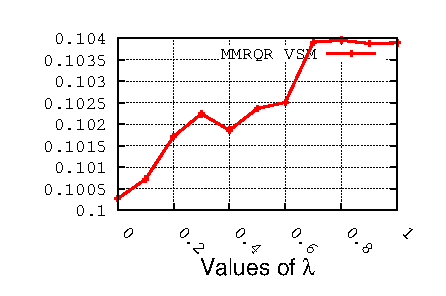
\includegraphics[width=4.3cm]{mmrqrResults-lambda/qAbstract-sDescription_MAP_2010}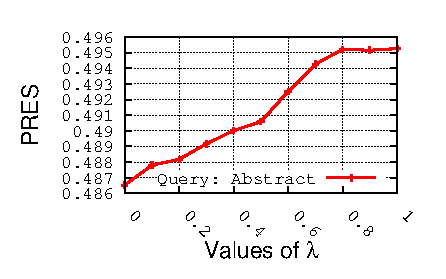
\includegraphics[width=4.3cm]{mmrqrResults-lambda/qAbstract-sDescription_PRES_2010}
\par\end{centering}

\begin{centering}
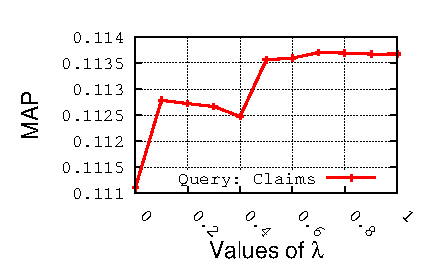
\includegraphics[width=4.3cm]{mmrqrResults-lambda/qClaims-sDescription_MAP_2010}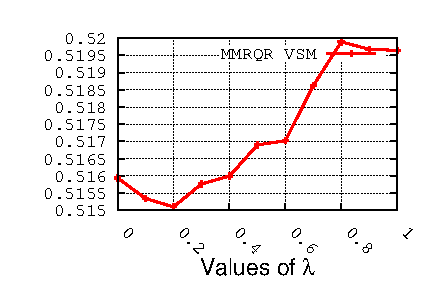
\includegraphics[width=4.3cm]{mmrqrResults-lambda/qClaims-sDescription_PRES_2010}
\par\end{centering}

\caption{Impact of the diversity parameter $\lambda$ on the performance of
MMRQR on the CLEF-IP 2010 dataset.}


\label{fig:DivImpactMMRQR}

\end{figure}


Next, we carry out experiments along the dimensions outlined in Section~\ref{sec:FrameworkQR}
with the following specific options:
\begin{itemize}
\item \textbf{\footnotesize{}Query type:}{\footnotesize{} $\{\mathrm{Title},\mathrm{Abstract},\mathrm{Claims},\mathrm{Description}\}$ }{\footnotesize \par}
\item \textbf{\footnotesize{}Relevance model:}{\footnotesize{} $\{\mathrm{BM25},\mbox{Vector-space Model (VSM)}\}$ }{\footnotesize \par}
\item \textbf{\footnotesize{}Term selection method:}{\footnotesize{} $\{\mathrm{RocchioQR},\mathrm{MMRQR},etc...\}$ }{\footnotesize \par}
\end{itemize}
Figure \ref{fig:QR-qDescription-CLEF-2010} shows the results obtained
in terms of MAP and PRES for CLEF-IP 2010 for different numbers of
removed terms $k$ on the x-axis (with $k=0$ using no QR, just the
baseline retrieval model). For lack of space we show only the results
of queries extracted from the description. These results tell us mainly
two things: (i) for the two retrieval models, MMRQR provides the best
performance for both MAP and PRES, and (ii) for both almost all methods,
the best performance is obtained when removing about 30 terms from
the original queries (in the case where the description is used for
querying). Removing more terms will decrease significantly the performance.

To summarize all the results obtained over all the above configurations,
Figures~\ref{fig:QR-PRES-CLEF-IP2010}, ~\ref{fig:QR-MAP-CLEF-IP2010},~\ref{fig:QR-PRES-CLEF-IP2011},
and~\ref{fig:QR-MAP-CLEF-IP2011} show the performance obtained for
all the QR methods, when selecting the optimal number of terms removed
from the original queries (number of terms removed that maximizes
the performance for each method). 

From these results, we make the following observations: (i) query
reduction is very often not useful for short queries (i.e. title),
since no QR method outperforms significantly the baseline (i.e. No
QR), (ii) when dealing with very long query (i.e. description), BM25
based QR methods perform better than VSM based QR methods, and (iii)
in general, MMRQR provides better performance than the other methods. 

To give an insight of the effect of MMRQR and LMQR over the performance,
Table \ref{tbl:QRSampleQueries} shows some queries where QR methods
improved the performance. First, we notice that even if there is common
terms removed from the original queries by both MMRQR and LMQR, the
lists of MMRQR contain more similar terms (e.g. \textit{laser, light,
interferometer} for the first example). For the two first examples,
for MMRQR, similar terms were removed from the queries, which favor
finding more diverse patent relevant to the patent applications. However,
for the third query, MMRQR removed the main terms from the query (\textit{motor},
and thermal \textit{load}), which probably decrease the quality of
the query. 

\begin{table*}[t]
\caption{Samples of queries extracted from CLEF-IP 2011, where MMRQR improves
the performance. (P: Precision, R: Recall, RR: Reciprocal Rank, AP:
Average Precision, PRES: Patent Retrieval Evaluation Score). MMRQR
improves the two first examples, while LMQR improves the third. }
\label{tbl:QRSampleQueries}

\centering{}%
\begin{tabular}{|>{\raggedright}p{17.5cm}|}
\hline 
\textbf{\scriptsize{}1- Topic: }{\scriptsize{}EP-1424597-A2}\tabularnewline
\hline 
\textbf{\scriptsize{}Abstract:}{\scriptsize{} Measurements of an interferometric
measurement system are corrected for variations of atmospheric conditions
such as pressure, temperature and turbulence using measurements from
a second harmonic interferometer (10). A ramp, representing the dependence
of the SHI data on path length, is removed before use of the SHI data.
The SHI may use a passive Q-switched laser (11) as a light source
and Brewster prisms (142,144) in the receiver module. Optical fibers
may be used to conduct light to the detectors (145-147). A mirror
reflecting the measurement beams has a coating of a thickness selected
to minimize the sensitivity of the SHI data to changes in coating
thickness.}\tabularnewline
\hline 
\begin{tabular}{>{\centering}p{16.5cm}}
{\scriptsize{}Baseline performance:}~{\scriptsize{}}%
\begin{tabular}{|c|c|c|c|c|c|c|c|c|c|c|c|}
\hline 
\textbf{\scriptsize{}P@5:} & {\scriptsize{}0.000} & \textbf{\scriptsize{}P@10:} & {\scriptsize{}0.000} & \textbf{\scriptsize{}R@10:} & {\scriptsize{}0.000} & \textbf{\scriptsize{}RR:} & {\scriptsize{}0.037} & \textbf{\scriptsize{}AP:} & {\scriptsize{}0.022} & \textbf{\scriptsize{}PRES:} & {\scriptsize{}0.648}\tabularnewline
\hline 
\end{tabular}\tabularnewline
\end{tabular}\tabularnewline
\hline 
\textbf{\scriptsize{}MMRQR removed terms: temperatur}{\scriptsize{},
}\textbf{\scriptsize{}detector}{\scriptsize{}, }\textbf{\scriptsize{}path}{\scriptsize{},
}\textbf{\scriptsize{}laser}{\scriptsize{}, }\textbf{\scriptsize{}light}{\scriptsize{},
}\textbf{\scriptsize{}interferometr}{\scriptsize{}, }\textbf{\scriptsize{}brewster}{\scriptsize{},
}\textbf{\scriptsize{}sensit}{\scriptsize{}, }\textbf{\scriptsize{}repres}{\scriptsize{},
}\textbf{\scriptsize{}sourc}\tabularnewline
\hline 
\begin{tabular}{>{\centering}p{16.5cm}}
{\scriptsize{}MMRQR performance:}~{\scriptsize{}}%
\begin{tabular}{|c|c|c|c|c|c|c|c|c|c|c|c|}
\hline 
\textbf{\scriptsize{}P@5:} & {\scriptsize{}0.000} & \textbf{\scriptsize{}P@10:} & {\scriptsize{}0.100} & \textbf{\scriptsize{}R@10:} & {\scriptsize{}0.166} & \textbf{\scriptsize{}RR:} & {\scriptsize{}0.111} & \textbf{\scriptsize{}AP:} & {\scriptsize{}0.053} & \textbf{\scriptsize{}PRES:} & {\scriptsize{}0.761}\tabularnewline
\hline 
\end{tabular}\tabularnewline
\end{tabular}\tabularnewline
\hline 
\textbf{\scriptsize{}LMQR removed terms: }{\scriptsize{}\uline{minim}}{\scriptsize{},
}{\scriptsize{}\uline{conduct}}{\scriptsize{}, }{\scriptsize{}\uline{variat}}{\scriptsize{},
}{\scriptsize{}\uline{shi}}{\scriptsize{}, }{\scriptsize{}\uline{turbul}}{\scriptsize{},
}{\scriptsize{}\uline{condit}}{\scriptsize{}, }{\scriptsize{}\uline{pressur}}{\scriptsize{},
}{\scriptsize{}\uline{remov}}{\scriptsize{}, }{\scriptsize{}\uline{ramp}}{\scriptsize{},
}{\scriptsize{}\uline{thick}}\tabularnewline
\hline 
\begin{tabular}{>{\centering}p{16.5cm}}
{\scriptsize{}LMQR performance:}~{\scriptsize{}}%
\begin{tabular}{|c|c|c|c|c|c|c|c|c|c|c|c|}
\hline 
\textbf{\scriptsize{}P@5:} & {\scriptsize{}0.000} & \textbf{\scriptsize{}P@10:} & {\scriptsize{}0.000} & \textbf{\scriptsize{}R@10:} & {\scriptsize{}0.000} & \textbf{\scriptsize{}RR:} & {\scriptsize{}0.076} & \textbf{\scriptsize{}AP:} & {\scriptsize{}0.036} & \textbf{\scriptsize{}PRES:} & {\scriptsize{}0.724}\tabularnewline
\hline 
\end{tabular}\tabularnewline
\end{tabular}\tabularnewline
\hline 
\hline 
\textbf{\scriptsize{}2- Topic: }{\scriptsize{}EP-1498393-A1}\tabularnewline
\hline 
\textbf{\scriptsize{}Abstract:}{\scriptsize{} In methods for recovering
and recycling helium and unreacted chlorine from a process for manufacturing
optical fiber an exhaust gas is recovered typically from a consolidation
furnace and is separated into helium-rich and chlorine-rich gas streams.
The helium-rich stream is typically dried and blended with make-up
helium and the chlorine-rich stream is typically purified and blended
with make-up chlorine so that both may be reused in the optical fiber
production process.}\tabularnewline
\hline 
\begin{tabular}{>{\centering}p{16.5cm}}
{\scriptsize{}Baseline performance:}~{\scriptsize{}}%
\begin{tabular}{|c|c|c|c|c|c|c|c|c|c|c|c|}
\hline 
\textbf{\scriptsize{}P@5:} & {\scriptsize{}0.200} & \textbf{\scriptsize{}P@10:} & {\scriptsize{}0.100} & \textbf{\scriptsize{}R@10:} & {\scriptsize{}0.125} & \textbf{\scriptsize{}RR:} & {\scriptsize{}0.200} & \textbf{\scriptsize{}AP:} & {\scriptsize{}0.060} & \textbf{\scriptsize{}PRES:} & {\scriptsize{}0.481}\tabularnewline
\hline 
\end{tabular}\tabularnewline
\end{tabular}\tabularnewline
\hline 
\textbf{\scriptsize{}MMRQR removed terms: stream}{\scriptsize{}, }\textbf{\scriptsize{}\uline{rich}}{\scriptsize{},
}\textbf{\scriptsize{}fiber}{\scriptsize{}, }\textbf{\scriptsize{}\uline{reus}}{\scriptsize{},
}\textbf{\scriptsize{}\uline{product}}{\scriptsize{}, }\textbf{\scriptsize{}\uline{dri}}{\scriptsize{},
}\textbf{\scriptsize{}separ}{\scriptsize{}, }\textbf{\scriptsize{}exhaust}{\scriptsize{},
}\textbf{\scriptsize{}\uline{method}}{\scriptsize{}, }\textbf{\scriptsize{}\uline{make}}\tabularnewline
\hline 
\begin{tabular}{>{\centering}p{16.5cm}}
{\scriptsize{}MMRQR performance:}~{\scriptsize{}}%
\begin{tabular}{|c|c|c|c|c|c|c|c|c|c|c|c|}
\hline 
\textbf{\scriptsize{}P@5:} & {\scriptsize{}0.200} & \textbf{\scriptsize{}P@10:} & {\scriptsize{}0.200} & \textbf{\scriptsize{}R@10:} & {\scriptsize{}0.250} & \textbf{\scriptsize{}RR:} & {\scriptsize{}0.250} & \textbf{\scriptsize{}AP:} & {\scriptsize{}0.106} & \textbf{\scriptsize{}PRES:} & {\scriptsize{}0.604}\tabularnewline
\hline 
\end{tabular}\tabularnewline
\end{tabular}\tabularnewline
\hline 
\textbf{\scriptsize{}LMQR removed terms: }\textbf{\scriptsize{}\uline{dri}}{\scriptsize{},
}\textbf{\scriptsize{}\uline{rich}}{\scriptsize{}, }{\scriptsize{}\uline{process}}{\scriptsize{},
}\textbf{\scriptsize{}\uline{product}}{\scriptsize{}, }\textbf{\scriptsize{}\uline{make}}{\scriptsize{},
}\textbf{\scriptsize{}\uline{reus}}{\scriptsize{}, }{\scriptsize{}\uline{unreact}}{\scriptsize{},
}{\scriptsize{}\uline{typic}}{\scriptsize{}, }{\scriptsize{}\uline{blend}}{\scriptsize{},
}\textbf{\scriptsize{}\uline{method}}{\scriptsize{}, }\tabularnewline
\hline 
\begin{tabular}{>{\centering}p{16.5cm}}
{\scriptsize{}LMQR performance:}~{\scriptsize{}}%
\begin{tabular}{|c|c|c|c|c|c|c|c|c|c|c|c|}
\hline 
\textbf{\scriptsize{}P@5:} & {\scriptsize{}0.200} & \textbf{\scriptsize{}P@10:} & {\scriptsize{}0.200} & \textbf{\scriptsize{}R@10:} & {\scriptsize{}0.250} & \textbf{\scriptsize{}RR:} & {\scriptsize{}0.200} & \textbf{\scriptsize{}AP:} & {\scriptsize{}0.097} & \textbf{\scriptsize{}PRES:} & {\scriptsize{}0.552}\tabularnewline
\hline 
\end{tabular}\tabularnewline
\end{tabular}\tabularnewline
\hline 
\hline 
\textbf{\scriptsize{}3- Topic: }{\scriptsize{}EP-1314594-A1}\tabularnewline
\hline 
\textbf{\scriptsize{}Abstract:}{\scriptsize{} An air conditioner for
air conditioning the interior of a compartment includes a compressor
(C) and an electric motor (84). The compressor (C) compresses refrigerant
gas and changes the displacement. The electric motor (84) drives the
compressor (C). A motor controller (72) rotates the motor (84) at
a constant reference speed. A detection device (92) detects information
related to the thermal load on the air conditioner. A current sensor
(97) detects the value of current supplied to the electric motor.
A controller (72) controls the compressor based on the detected thermal
load information and the detected current value. The controller (72)
computes a target torque of the compressor based on the thermal load
information. In accordance with the computed target torque, the controller
(72) computes a target current value to be supplied to the electric
motor. The controller (72) further controls the displacement of the
compressor such that the detected current value matches the target
current value.}\tabularnewline
\hline 
\begin{tabular}{>{\centering}p{16.5cm}}
{\scriptsize{}Baseline performance:}~{\scriptsize{}}%
\begin{tabular}{|c|c|c|c|c|c|c|c|c|c|c|c|}
\hline 
\textbf{\scriptsize{}P@5:} & {\scriptsize{}0.600} & \textbf{\scriptsize{}P@10:} & {\scriptsize{}0.400} & \textbf{\scriptsize{}R@10:} & {\scriptsize{}0.307} & \textbf{\scriptsize{}RR:} & {\scriptsize{}1.000} & \textbf{\scriptsize{}AP:} & {\scriptsize{}0.301} & \textbf{\scriptsize{}PRES:} & {\scriptsize{}0.777}\tabularnewline
\hline 
\end{tabular}\tabularnewline
\end{tabular}\tabularnewline
\hline 
\textbf{\scriptsize{}MMRQR removed terms:}{\scriptsize{} }\textbf{\scriptsize{}\uline{refer}}{\scriptsize{},
}\textbf{\scriptsize{}motor}{\scriptsize{}, }\textbf{\scriptsize{}\uline{current}}{\scriptsize{},
}\textbf{\scriptsize{}\uline{relat}}{\scriptsize{}, }\textbf{\scriptsize{}condit}{\scriptsize{},
}\textbf{\scriptsize{}constant}{\scriptsize{}, }\textbf{\scriptsize{}\uline{suppli}}{\scriptsize{},
}\textbf{\scriptsize{}\uline{compress}}{\scriptsize{}, }\textbf{\scriptsize{}load}{\scriptsize{},
}\textbf{\scriptsize{}\uline{match}}\tabularnewline
\hline 
\begin{tabular}{>{\centering}p{16.5cm}}
{\scriptsize{}MMRQR performance:}~{\scriptsize{}}%
\begin{tabular}{|c|c|c|c|c|c|c|c|c|c|c|c|}
\hline 
\textbf{\scriptsize{}P@5:} & {\scriptsize{}0.400} & \textbf{\scriptsize{}P@10:} & {\scriptsize{}0.500} & \textbf{\scriptsize{}R@10:} & {\scriptsize{}0.384} & \textbf{\scriptsize{}RR}{\scriptsize{}:} & {\scriptsize{}0.500} & \textbf{\scriptsize{}AP:} & {\scriptsize{}0.221} & \textbf{\scriptsize{}PRES:} & {\scriptsize{}0.774}\tabularnewline
\hline 
\end{tabular}\tabularnewline
\end{tabular}\tabularnewline
\hline 
\textbf{\scriptsize{}LMQR removed terms: }{\scriptsize{}\uline{compart}}{\scriptsize{},
}\textbf{\scriptsize{}\uline{suppli}}{\scriptsize{}, }\textbf{\scriptsize{}\uline{current}}{\scriptsize{},
}{\scriptsize{}\uline{ga}}{\scriptsize{}, }\textbf{\scriptsize{}\uline{refer}}{\scriptsize{},
}\textbf{\scriptsize{}\uline{compress}}{\scriptsize{}, }\textbf{\scriptsize{}\uline{relat}}{\scriptsize{},
}{\scriptsize{}\uline{interior}}{\scriptsize{}, }{\scriptsize{}\uline{thermal}}{\scriptsize{},
}\textbf{\scriptsize{}\uline{match}}{\scriptsize{}, }\tabularnewline
\hline 
\begin{tabular}{>{\centering}p{16.5cm}}
{\scriptsize{}LMQR performance:}~{\scriptsize{}}%
\begin{tabular}{|c|c|c|c|c|c|c|c|c|c|c|c|}
\hline 
\textbf{\scriptsize{}P@5:} & {\scriptsize{}0.400} & \textbf{\scriptsize{}P@10:} & {\scriptsize{}0.400} & \textbf{\scriptsize{}R@10:} & {\scriptsize{}0.307} & \textbf{\scriptsize{}RR:} & {\scriptsize{}1.000} & \textbf{\scriptsize{}AP:} & {\scriptsize{}0.266} & \textbf{\scriptsize{}PRES:} & {\scriptsize{}0.802}\tabularnewline
\hline 
\end{tabular}\tabularnewline
\end{tabular}\tabularnewline
\hline 
\end{tabular}
\end{table*}


%\section{Related Work}
%\label{sec:relatedworks}


%The major contributions in patent search has focused on query formulation, where the objective is to find the best terms to represent a patent application as a query to achieve high retrieval effectiveness by retrieving all possible relevant documents at high ranks \cite{Magdy2012}. 


%The scenario of patent prior art search consists of manually form queries by selecting high frequency terms from patent application. Hence, following this methodology, some algorithms of patent query reduction have been proposed to select only useful terms from patent application \cite{Ganguly2011,Itoh2003}. We used the approach propose by Ganguly et al. \cite{Ganguly2011} for QR as a baseline, and we showed that the performance of MMRQR outperform this approach in many cases. 


%The major contributions in patent search has focused on query formulation, where the objective is to find the best terms to represent a patent application as a query to achieve high retrieval effectiveness by retrieving all possible relevant documents at high ranks \cite{Magdy2012}.


\begin{comment}
There are a variety of existing query expansion methods that use synonyms
(both from WordNet and automatically generated)~\cite{Magdy2011},
by supervised learning~\cite{Bashir2010}, by IPC codes (a variant
on our baseline approach that additionally uses the citation network
of patents)~\cite{Verma2011}, and a query-specific patent lexicon
based on the definitions of the IPC~\cite{Mahdabi2013}. While our
intention in this paper was to comprehensively evaluate very general
methods for QE using \emph{partial patent applications}; it would
be interesting future work to comprehensively evaluate all of these
patent-specific QE methods with our generic methods for partial patent
application queries. 
\end{comment}


%Classical query expansion methods has been used for prior art search by 
%Magdy et al. \cite{Magdy2011}, which rely on pseudo-relevance feedback and WordNet as
%source of expansion terms. However, none of these approaches were
%able to achieve a significant improvement over the baseline. Therefore,
%they introduce a novel approach that automatically generates synonym
%sets for terms, and use them as a source of expansion terms, which
%showed significant improvement with respect to the baseline. 
%Also, Bashir et al. \cite{Bashir2010} propose a query expansion with pseudo-relevance
%feedback. Query expansion terms are selected using a using a machine
%learning approach, by picking terms that may have a potential positive
%impact on the retrieval effectiveness. However, this approach can
%be computational expensive, since the presented features are complicated
%to compute, e.g. Pair-wise Terms Proximity features. 
%Verma and Varma \cite{Verma2011} propose a different approach, which instead of using
%the patent text to query, use its International Patent Classification
%(IPC) codes, which are expanded using the citation network. The formed
%query is used to perform an initial search. The results are then re-ranked
%using queries constructed from patent text. Throughout our experiments,
%we concluded that relying on non-patent terms to expand a query, leads to poor retrieval quality.
%Lastly, a more recent work by Mahdabi et al. \cite{Mahdabi2013} propose to combine query reduction and expansion method for prior art search.
%For query reduction, they shorten the query by taking only the first claim since it contains the core of the invention.
%For the query expansion, they built a query-specific patent lexicon based on the definitions of the IPC. Then, 
%the patent lexicon is used to
%select expansion terms that are focused on the reduced query.


%Others investigated query suggestion for patent prior
%art search, which reflect real-life scenario of examiners, who form
%reproducible boolean queries \cite{Adams2011,Azzopardi2010,Kim2011}. 
%In this paper, we focus on generic query expansion methods, but it would be interesting to apply the founded insights 
%to improve patent search specific strategies as the ones just mentioned.


%Finally, also query reduction methods have been applied in order to deal with long queries, which are composed by full patent applications \cite{Ganguly2011,Itoh2003}. Even these methods are interesting, they are not suited to deal with short queries (partial patent applications).


\begin{center}
\begin{figure}[t]
\begin{centering}
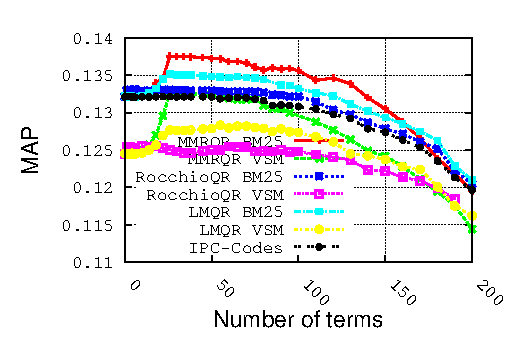
\includegraphics[width=4.3cm]{mmrqrResults/qDescription-sDescription_MAP_2010}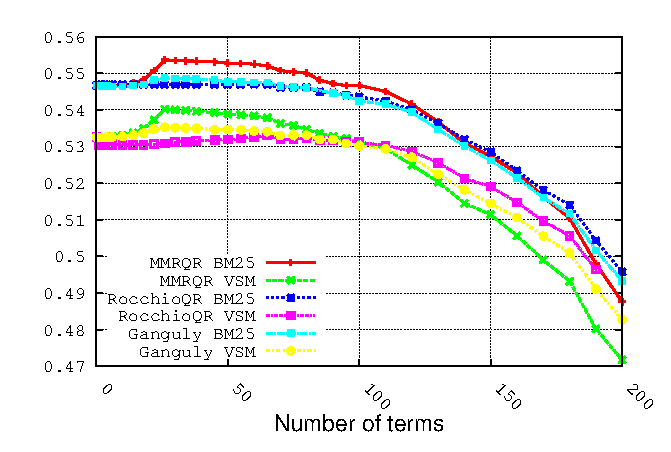
\includegraphics[width=4.3cm]{mmrqrResults/qDescription-sDescription_PRES_2010}
\par\end{centering}

\caption{Results obtained for QR while using the description for querying on
the CLEF-IP 2010 dataset.}


\label{fig:QR-qDescription-CLEF-2010}
\end{figure}

\par\end{center}


\section{Conclusion}

\label{sec:conclusion}

In this paper we analyzed general and specific QE and QR methods for
patent prior art search with incomplete patent applications on two
patent retrieval corpora, namely CLEF-IP 2010 and CLEF-IP 2011. We
demonstrated that QE methods are critical for short queries, i.e.
title, abstract, and claims, but useless for very long queries, i.e.
the description section. We also showed that claims are the best section
that works with QE both to query with and to use as a source of query
expansion terms, and that a new method MMRQE improves QE results in
many cases. Future work can look at more patent-specific methods of
QE for prior art search with partial patent applications and how they
can be integrated with methods like MMRQE. 

Regarding QR methods, we showed that these techniques are effective
to some extend for claims and description sections, which are considered
as the longest sections in a patent application. We also demonstrated
that our new QR method MMRQR might improve both recall and precision
in many cases. For this second part, future work may consist of exploiting
query quality predictors to identify useless terms in a query using
machine learning methods. 

%We demonstrated that it reasonable to do prior art search 
%with partial applications, especially when combined with query expansion methods. 
%We also found that the patent specific fields are more suited as a source for expansion than other sources.
%We plan to further refine our approach by using
%a term weighting scheme for MMRQE. Other future work direction is to used MMR
%during query reduction to remove terms, which are not diversified
%in the query.




{ \scriptsize

\bibliographystyle{abbrv}
\bibliography{biblio}


}

\clearpage{}

\begin{figure*}[t]
\begin{centering}
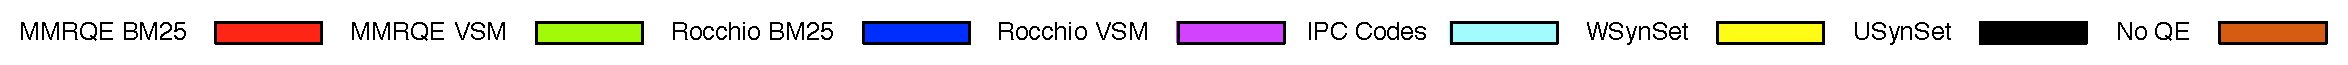
\includegraphics[width=17cm]{img/legendQE}
\par\end{centering}

\begin{centering}
\subfigure[{\tiny Query Title.}]{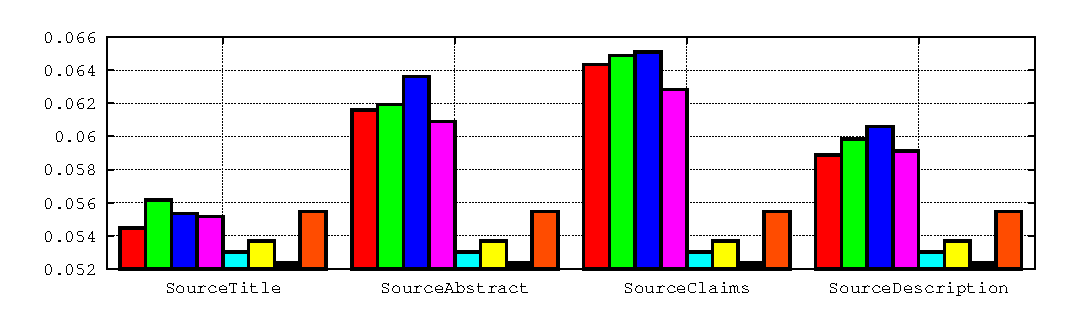
\includegraphics[width=8.6cm]{Results-CIKM2014/qTitle-MAP-CLEF-IP2010}}\subfigure[{\tiny Query Abstract.}]{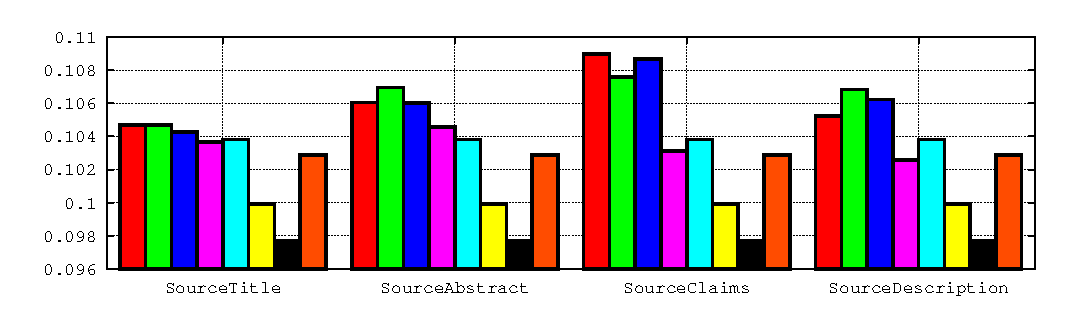
\includegraphics[width=8.6cm]{Results-CIKM2014/qAbstract-MAP-CLEF-IP2010}}
\par\end{centering}

\begin{centering}
\subfigure[{\tiny Query Claims.}]{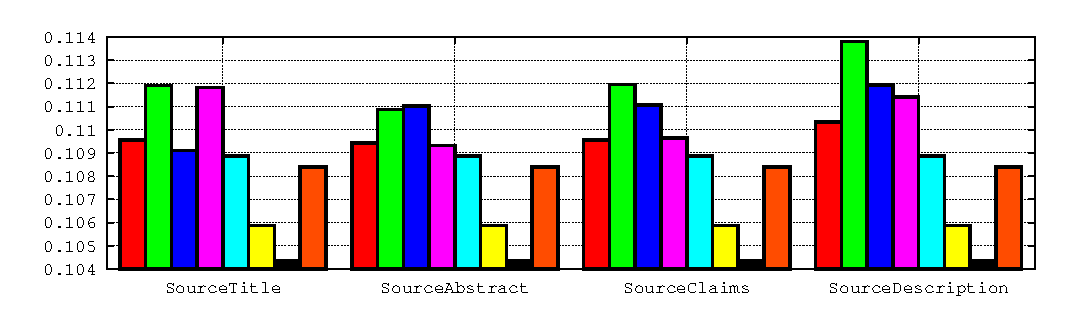
\includegraphics[width=8.6cm]{Results-CIKM2014/qClaims-MAP-CLEF-IP2010}}\subfigure[{\tiny Query Description.}]{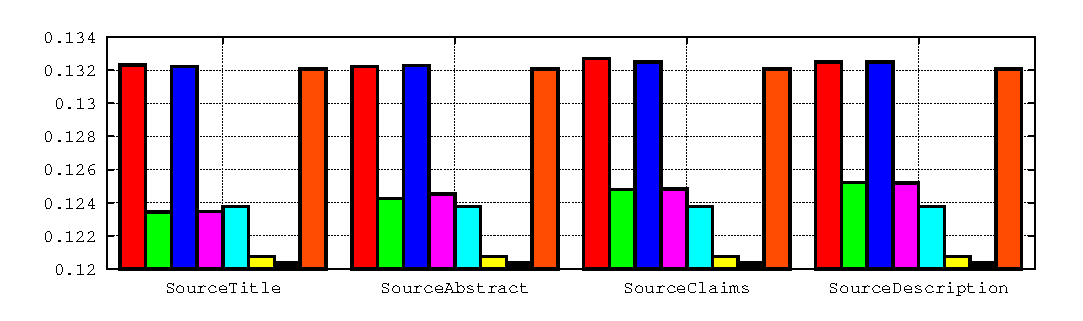
\includegraphics[width=8.6cm]{Results-CIKM2014/qDescription-MAP-CLEF-IP2010}\label{fig:qDescription-MAP-CLEF-IP2010}}
\par\end{centering}

\caption{Mean Average Precision (MAP) for QE methods on CLEF-2010 (for MMRQE
$\lambda=0.5$).}


\label{fig:MAP-CLEF2010}
\end{figure*}


\begin{figure*}[t]
\begin{centering}
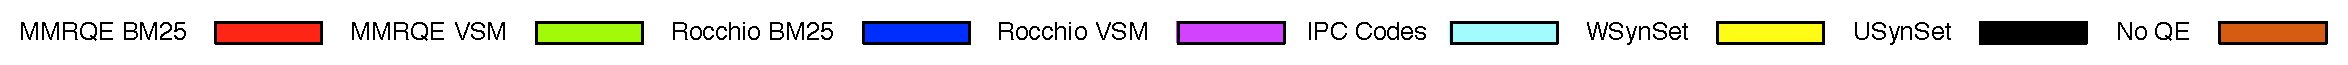
\includegraphics[width=17cm]{img/legendQE}
\par\end{centering}

\begin{centering}
\subfigure[{\tiny Query Title.}]{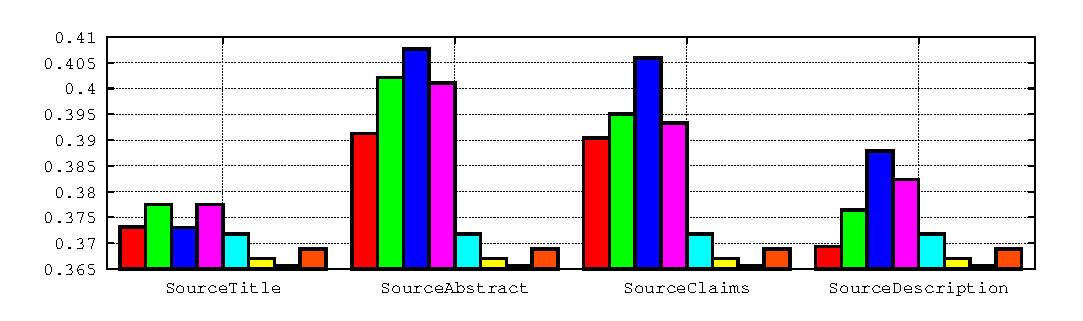
\includegraphics[width=8.6cm]{Results-CIKM2014/qTitle-PRES-CLEF-IP2010}}\subfigure[{\tiny Query Abstract.}]{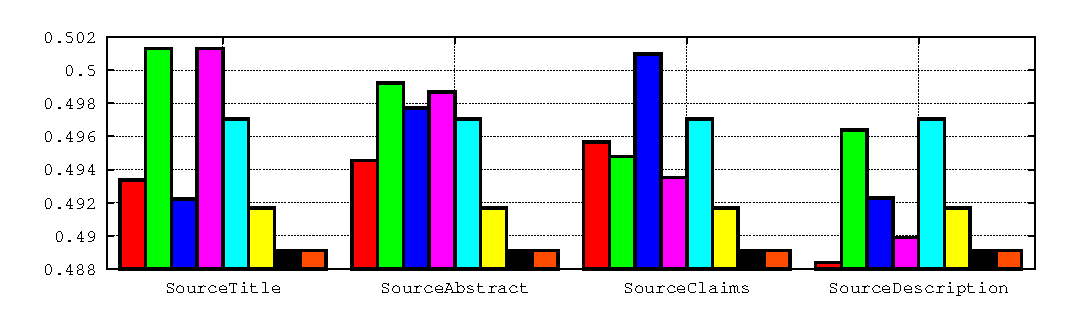
\includegraphics[width=8.6cm]{Results-CIKM2014/qAbstract-PRES-CLEF-IP2010}}
\par\end{centering}

\begin{centering}
\subfigure[{\tiny Query Claims.}]{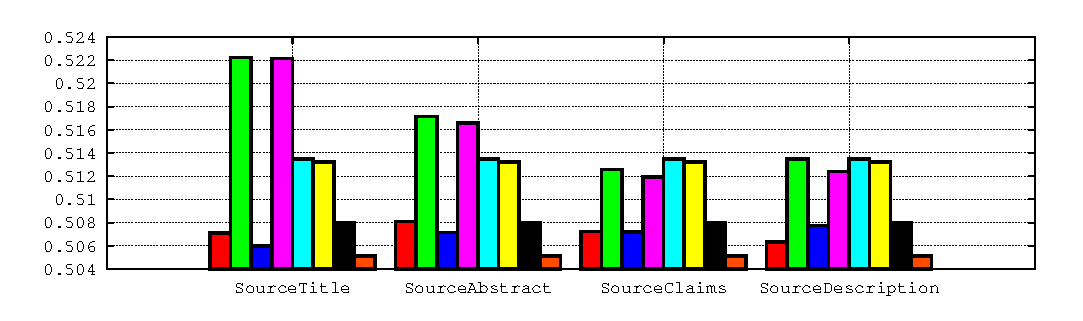
\includegraphics[width=8.6cm]{Results-CIKM2014/qClaims-PRES-CLEF-IP2010}}\subfigure[{\tiny Query Description.}]{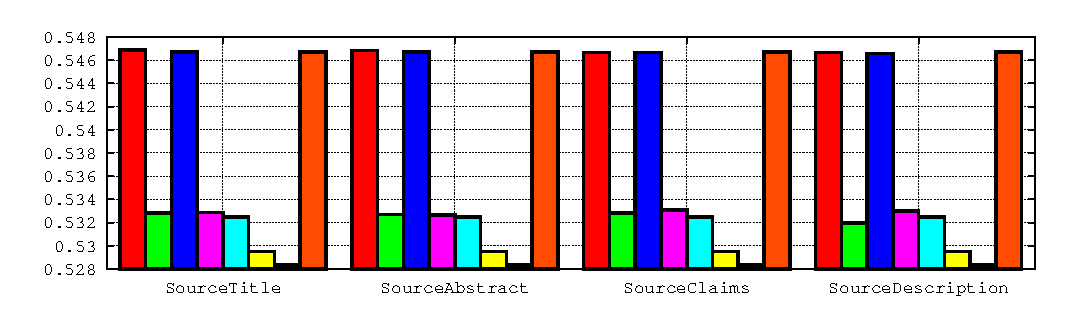
\includegraphics[width=8.6cm]{Results-CIKM2014/qDescription-PRES-CLEF-IP2010}\label{fig:qDescription-PRES-CLEF-IP2010}} 
\par\end{centering}

\caption{Patent Retrieval Evaluation Score (PRES) for QE methods on CLEF-2010
(for MMRQE $\lambda=0.5$).}


\label{fig:PRES-CLEF2010}
\end{figure*}


\begin{figure*}[t]
\begin{centering}
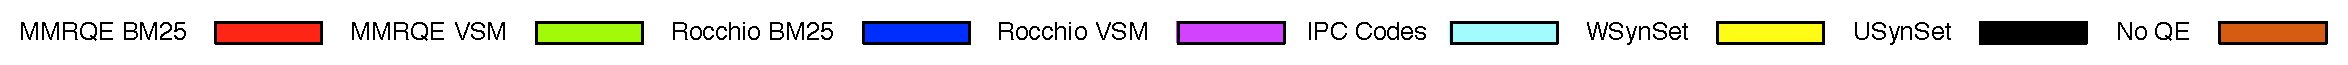
\includegraphics[width=17cm]{img/legendQE}
\par\end{centering}

\begin{centering}
\subfigure[{\tiny Query Title.}]{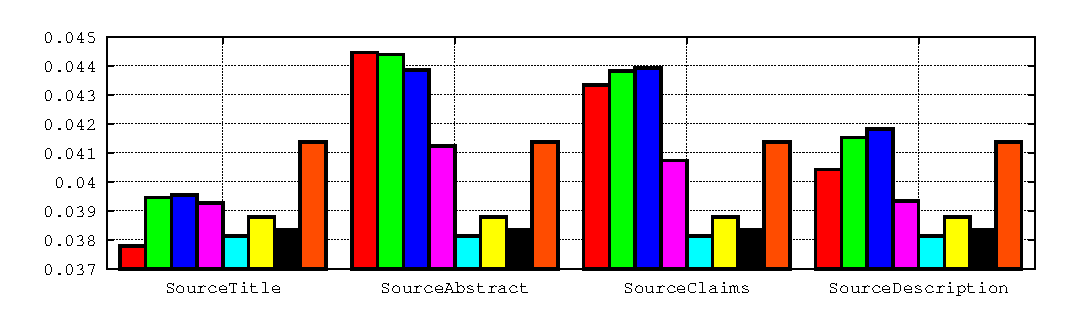
\includegraphics[width=8.6cm]{Results-CIKM2014/qTitle-MAP-CLEF-IP2011}}\subfigure[{\tiny Query Abstract.}]{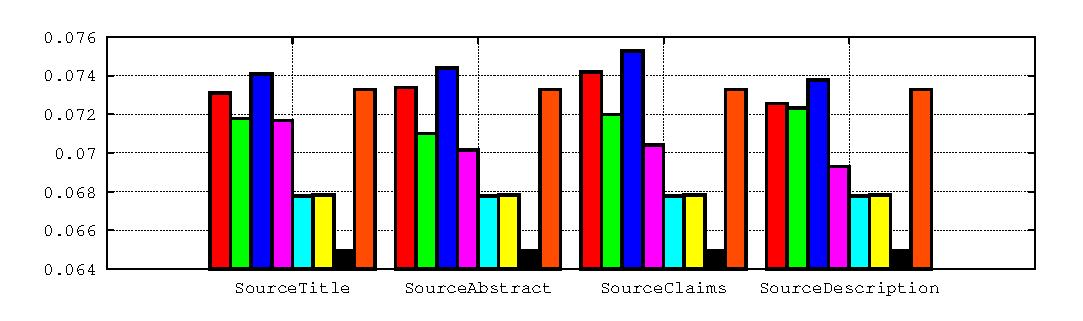
\includegraphics[width=8.6cm]{Results-CIKM2014/qAbstract-MAP-CLEF-IP2011}}
\par\end{centering}

\begin{centering}
\subfigure[{\tiny Query Claims.}]{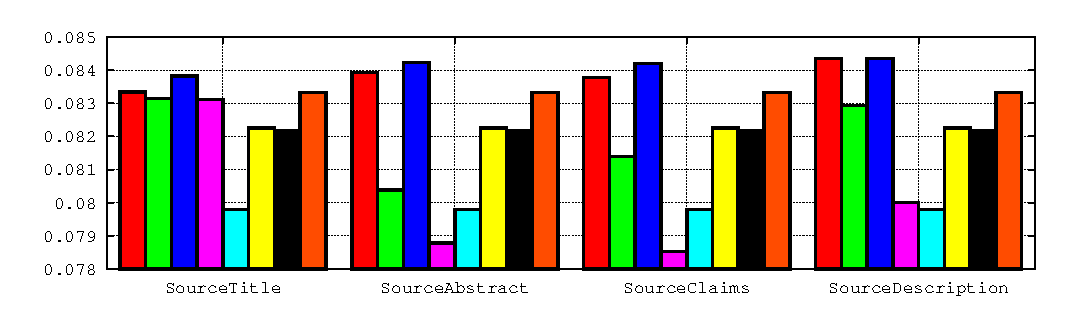
\includegraphics[width=8.6cm]{Results-CIKM2014/qClaims-MAP-CLEF-IP2011}}\subfigure[{\tiny Query Description.}]{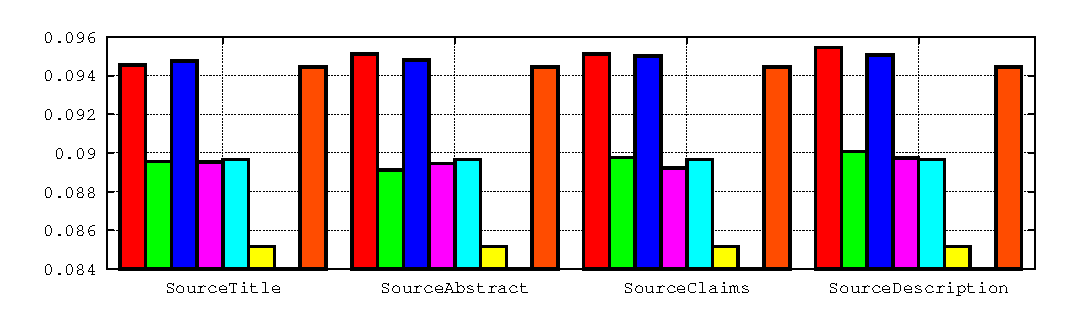
\includegraphics[width=8.6cm]{Results-CIKM2014/qDescription-MAP-CLEF-IP2011}\label{fig:qDescription-MAP-CLEF-IP2011}} 
\par\end{centering}

\caption{Mean Average Precision (MAP) for QE methods on CLEF-2011 (for MMRQE
$\lambda=0.5$).}


\label{fig:MAP-CLEF2011}
\end{figure*}


\clearpage{}

\begin{figure*}[t]
\begin{centering}
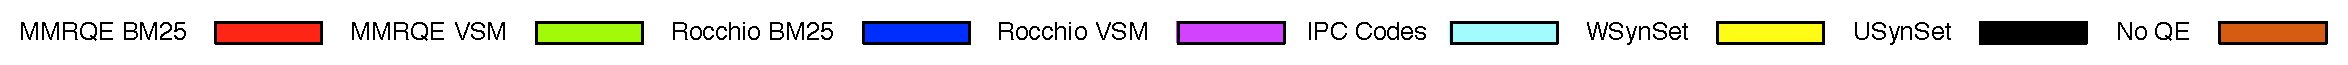
\includegraphics[width=17cm]{img/legendQE}
\par\end{centering}

\begin{centering}
\subfigure[{\tiny Query Title.}]{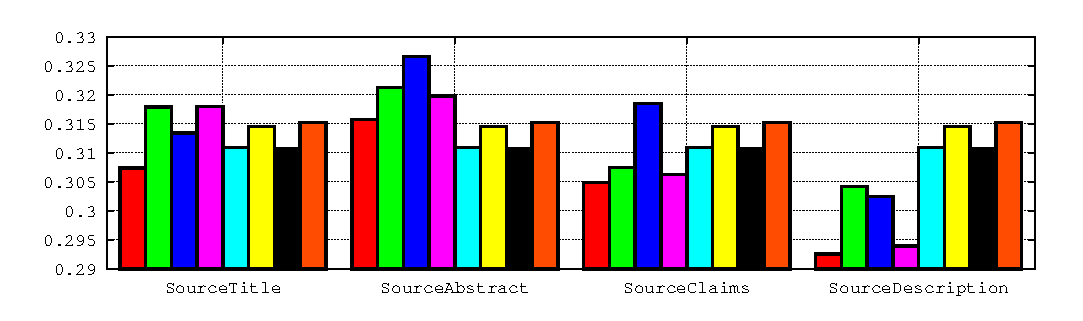
\includegraphics[width=8.4cm]{Results-CIKM2014/qTitle-PRES-CLEF-IP2011}}\subfigure[{\tiny Query Abstract.}]{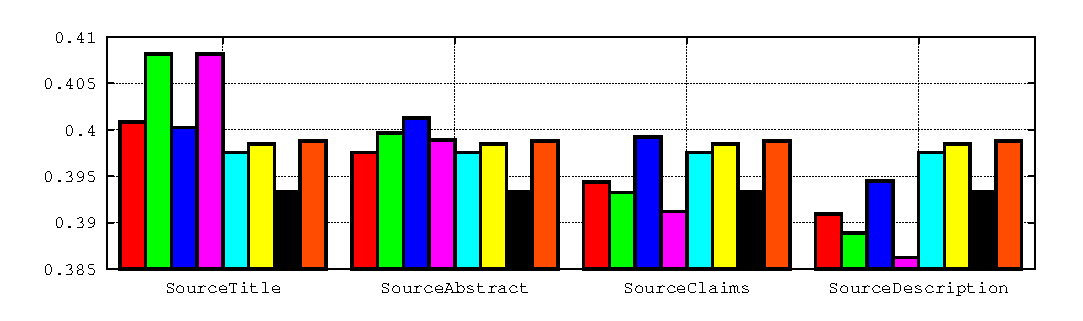
\includegraphics[width=8.4cm]{Results-CIKM2014/qAbstract-PRES-CLEF-IP2011}}
\par\end{centering}

\begin{centering}
\subfigure[{\tiny Query Claims.}]{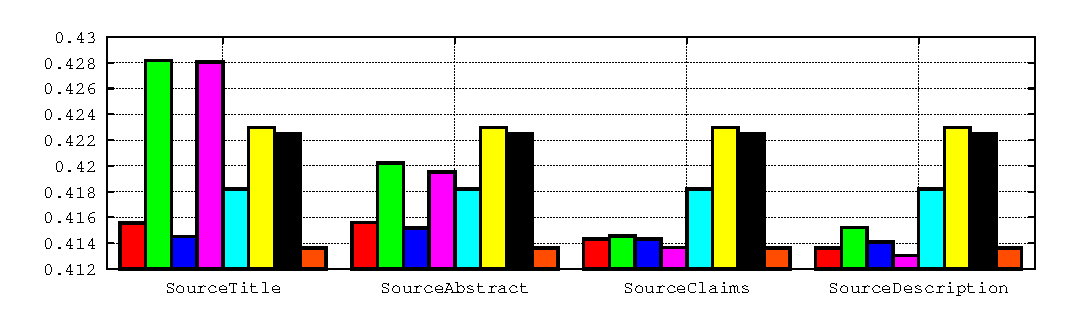
\includegraphics[width=8.4cm]{Results-CIKM2014/qClaims-PRES-CLEF-IP2011}}\subfigure[{\tiny Query Description.}]{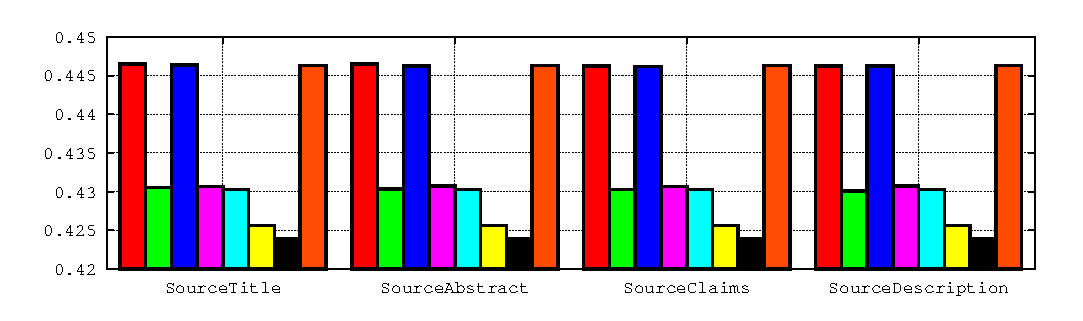
\includegraphics[width=8.6cm]{Results-CIKM2014/qDescription-PRES-CLEF-IP2011}\label{fig:qDescription-PRES-CLEF-IP2011}} 
\par\end{centering}

\caption{Patent Retrieval Evaluation Score (PRES) for QE methods on CLEF-2011
(for MMRQE $\lambda=0.5$).}


\label{fig:PRES-CLEF2011}
\end{figure*}


\begin{figure*}[t]
\begin{centering}
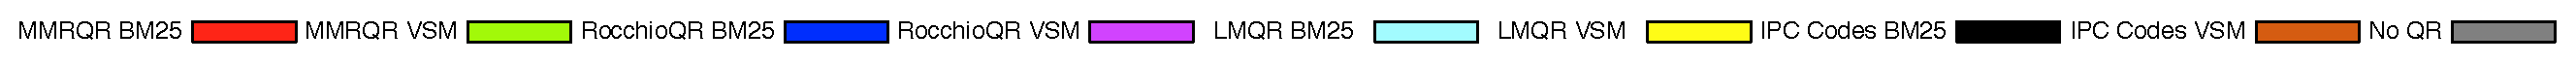
\includegraphics[width=15.5cm]{img/legendQR}
\par\end{centering}

\begin{centering}
\subfigure[{Query Title.}]{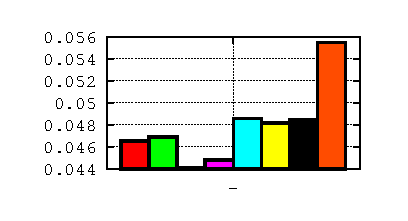
\includegraphics[width=4cm]{mmrqrResults/qTitle-MAP-CLEF-IP2010}}\subfigure[{Query Abstract.}]{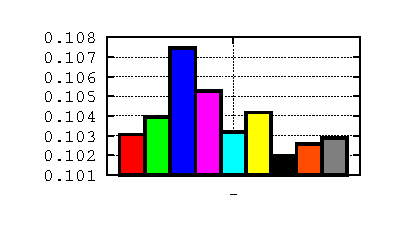
\includegraphics[width=4cm]{mmrqrResults/qAbstract-MAP-CLEF-IP2010}}\subfigure[{Query Claims.}]{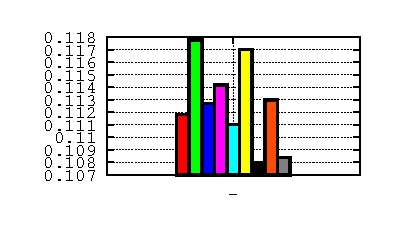
\includegraphics[width=4cm]{mmrqrResults/qClaims-MAP-CLEF-IP2010}}
\subfigure[{Query Description.}]{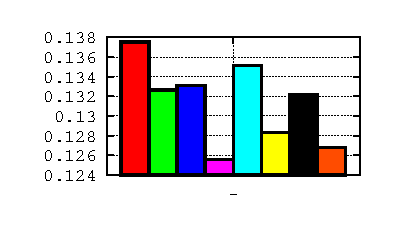
\includegraphics[width=4cm]{mmrqrResults/qDescription-MAP-CLEF-IP2010}} 
\par\end{centering}

\caption{Mean Average Precision (MAP) for QR methods on CLEF-2010 (for MMRQR
$\lambda=0.8$).}


\label{fig:QR-PRES-CLEF-IP2010}
\end{figure*}


\begin{figure*}[t]
\begin{centering}
\includegraphics[width=15.5cm]{img/legendQR}
\par\end{centering}

\begin{centering}
\subfigure[{Query Title.}]{\includegraphics[width=4cm]{mmrqrResults/qTitle-PRES-CLEF-IP2010}}\subfigure[{Query Abstract.}]{\includegraphics[width=4cm]{mmrqrResults/qAbstract-PRES-CLEF-IP2010}}\subfigure[{Query Claims.}]{\includegraphics[width=4cm]{mmrqrResults/qClaims-PRES-CLEF-IP2010}}
\subfigure[{Query Description.}]{\includegraphics[width=4cm]{mmrqrResults/qDescription-PRES-CLEF-IP2010}} 
\par\end{centering}

\caption{Patent Retrieval Evaluation Score (PRES) for QR methods on CLEF-2010
(for MMRQR $\lambda=0.8$).}


\label{fig:QR-MAP-CLEF-IP2010}
\end{figure*}


\begin{figure*}[t]
\begin{centering}
\includegraphics[width=15.5cm]{img/legendQR}
\par\end{centering}

\begin{centering}
\subfigure[{Query Title.}]{\includegraphics[width=4cm]{mmrqrResults/qTitle-MAP-CLEF-IP2011}}\subfigure[{Query Abstract.}]{\includegraphics[width=4cm]{mmrqrResults/qAbstract-MAP-CLEF-IP2011}}\subfigure[{Query Claims.}]{\includegraphics[width=4cm]{mmrqrResults/qClaims-MAP-CLEF-IP2011}}
\subfigure[{Query Description.}]{\includegraphics[width=4cm]{mmrqrResults/qDescription-MAP-CLEF-IP2011}} 
\par\end{centering}

\caption{Mean Average Precision (MAP) for QR methods on CLEF-2011 (for MMRQR
$\lambda=0.8$).}


\label{fig:QR-PRES-CLEF-IP2011}
\end{figure*}


\begin{figure*}[t]
\begin{centering}
\includegraphics[width=15.5cm]{img/legendQR}
\par\end{centering}

\begin{centering}
\subfigure[{Query Title.}]{\includegraphics[width=4cm]{mmrqrResults/qTitle-PRES-CLEF-IP2011}}\subfigure[{Query Abstract.}]{\includegraphics[width=4cm]{mmrqrResults/qAbstract-PRES-CLEF-IP2011}}\subfigure[{Query Claims.}]{\includegraphics[width=4cm]{mmrqrResults/qClaims-PRES-CLEF-IP2011}}
\subfigure[{Query Description.}]{\includegraphics[width=4cm]{mmrqrResults/qDescription-PRES-CLEF-IP2011}} 
\par\end{centering}

\caption{Patent Retrieval Evaluation Score (PRES) for QR methods on CLEF-2011
(for MMRQR $\lambda=0.8$).}


\label{fig:QR-MAP-CLEF-IP2011}
\end{figure*}


\clearpage{}

\begin{comment}
\begin{figure*}[t]
\begin{centering}
\subfigure[{\tiny Query Title \& source Title.}]{\includegraphics[width=4.3cm]{Results-CIKM2014/qTitle-sTitle_MAP_2010.eps}}\subfigure[{\tiny Query Title \& source Abstract.}]{\includegraphics[width=4.3cm]{Results-CIKM2014/qTitle-sAbstract_MAP_2010.eps}}\subfigure[{\tiny Query Title \& source Claims.}]{\includegraphics[width=4.3cm]{Results-CIKM2014/qTitle-sClaims_MAP_2010.eps}}\subfigure[{\tiny Query Title \& source Descrip.}]{\includegraphics[width=4.3cm]{Results-CIKM2014/qTitle-sDescription_MAP_2010.eps}} 
\par\end{centering}

\begin{centering}
\subfigure[{\tiny Query Abstract \& source Title.}]{\includegraphics[width=4.3cm]{Results-CIKM2014/qAbstract-sTitle_MAP_2010.eps}}\subfigure[{\tiny Query Abstract \& source Abstract.}]{\includegraphics[width=4.3cm]{Results-CIKM2014/qAbstract-sAbstract_MAP_2010.eps}}\subfigure[{\tiny Query Abstract \& source Claims.}]{\includegraphics[width=4.3cm]{Results-CIKM2014/qAbstract-sClaims_MAP_2010.eps}}\subfigure[{\tiny Query Abstract \& source Descrip.}]{\includegraphics[width=4.3cm]{Results-CIKM2014/qAbstract-sDescription_MAP_2010.eps}} 
\par\end{centering}

\begin{centering}
\subfigure[{\tiny Query Claims \& source Title.}]{\includegraphics[width=4.3cm]{Results-CIKM2014/qClaims-sTitle_MAP_2010.eps}}\subfigure[{\tiny Query Claims \& source Abstract.}]{\includegraphics[width=4.3cm]{Results-CIKM2014/qClaims-sAbstract_MAP_2010.eps}}\subfigure[{\tiny Query Claims \& source Claims.}]{\includegraphics[width=4.3cm]{Results-CIKM2014/qClaims-sClaims_MAP_2010.eps}}\subfigure[{\tiny Query Claims \& source Descrip.}]{\includegraphics[width=4.3cm]{Results-CIKM2014/qClaims-sDescription_MAP_2010.eps}}
\subfigure[{\tiny Query Descrip \& source Title.}]{\includegraphics[width=4.3cm]{Results-CIKM2014/qDescription-sTitle_MAP_2010.eps}}\subfigure[{\tiny Query Descrip \& source Abstract.}]{\includegraphics[width=4.3cm]{Results-CIKM2014/qDescription-sAbstract_MAP_2010.eps}}\subfigure[{\tiny Query Descrip \& source Claims.}]{\includegraphics[width=4.3cm]{Results-CIKM2014/qDescription-sClaims_MAP_2010.eps}}\subfigure[{\tiny Query Descrip \& source Descrip.}]{\includegraphics[width=4.3cm]{Results-CIKM2014/qDescription-sDescription_MAP_2010.eps}} 
\par\end{centering}

\caption{Mean Average Precision (MAP) on CLEF-2010 (for MMRQE $\lambda=0.5$).}


\label{fig:MAP-CLEF2010-1}
\end{figure*}


\begin{figure*}
\begin{centering}
\subfigure[{\tiny Query Title \& source Title.}]{\includegraphics[width=4.3cm]{Results-CIKM2014/qTitle-sTitle_PRES_2010.eps}}\subfigure[{\tiny Query Title \& source Abstract.}]{\includegraphics[width=4.3cm]{Results-CIKM2014/qTitle-sAbstract_PRES_2010.eps}}\subfigure[{\tiny Query Title \& source Claims.}]{\includegraphics[width=4.3cm]{Results-CIKM2014/qTitle-sClaims_PRES_2010.eps}}\subfigure[{\tiny Query Title \& source Descrip.}]{\includegraphics[width=4.3cm]{Results-CIKM2014/qTitle-sDescription_PRES_2010.eps}} 
\par\end{centering}

\begin{centering}
\subfigure[{\tiny Query Abstract \& source Title.}]{\includegraphics[width=4.3cm]{Results-CIKM2014/qAbstract-sTitle_PRES_2010.eps}}\subfigure[{\tiny Query Abstract \& source Abstract.}]{\includegraphics[width=4.3cm]{Results-CIKM2014/qAbstract-sAbstract_PRES_2010.eps}}\subfigure[{\tiny Query Abstract \& source Claims.}]{\includegraphics[width=4.3cm]{Results-CIKM2014/qAbstract-sClaims_PRES_2010.eps}}\subfigure[{\tiny Query Abstract \& source Descrip.}]{\includegraphics[width=4.3cm]{Results-CIKM2014/qAbstract-sDescription_PRES_2010.eps}} 
\par\end{centering}

\begin{centering}
\subfigure[{\tiny Query Claims \& source Title.}]{\includegraphics[width=4.3cm]{Results-CIKM2014/qClaims-sTitle_PRES_2010.eps}}\subfigure[{\tiny Query Claims \& source Abstract.}]{\includegraphics[width=4.3cm]{Results-CIKM2014/qClaims-sAbstract_PRES_2010.eps}}\subfigure[{\tiny Query Claims \& source Claims.}]{\includegraphics[width=4.3cm]{Results-CIKM2014/qClaims-sClaims_PRES_2010.eps}}\subfigure[{\tiny Query Claims \& source Descrip.}]{\includegraphics[width=4.3cm]{Results-CIKM2014/qClaims-sDescription_PRES_2010.eps}}
\subfigure[{\tiny Query Descrip \& source Title.}]{\includegraphics[width=4.3cm]{Results-CIKM2014/qDescription-sTitle_PRES_2010.eps}}\subfigure[{\tiny Query Descrip \& source Abstract.}]{\includegraphics[width=4.3cm]{Results-CIKM2014/qDescription-sAbstract_PRES_2010.eps}}\subfigure[{\tiny Query Descrip \& source Claims.}]{\includegraphics[width=4.3cm]{Results-CIKM2014/qDescription-sClaims_PRES_2010.eps}}\subfigure[{\tiny Query Descrip \& source Descrip.}]{\includegraphics[width=4.3cm]{Results-CIKM2014/qDescription-sDescription_PRES_2010.eps}} 
\par\end{centering}

\caption{Patent Retrieval Evaluation Score (PRES) on CLEF-2010 (for MMRQE $\lambda=0.5$).}


\label{fig:PRES-CLEF2010-1} 
\end{figure*}


\begin{figure*}[t]
\begin{centering}
\subfigure[{\tiny Query Title \& source Title.}]{\includegraphics[width=4.3cm]{Results-CIKM2014/qTitle-sTitle_MAP_2011.eps}}\subfigure[{\tiny Query Title \& source Abstract.}]{\includegraphics[width=4.3cm]{Results-CIKM2014/qTitle-sAbstract_MAP_2011.eps}}\subfigure[{\tiny Query Title \& source Claims.}]{\includegraphics[width=4.3cm]{Results-CIKM2014/qTitle-sClaims_MAP_2011.eps}}\subfigure[{\tiny Query Title \& source Descrip.}]{\includegraphics[width=4.3cm]{Results-CIKM2014/qTitle-sDescription_MAP_2011.eps}} 
\par\end{centering}

\begin{centering}
\subfigure[{\tiny Query Abstract \& source Title.}]{\includegraphics[width=4.3cm]{Results-CIKM2014/qAbstract-sTitle_MAP_2011.eps}}\subfigure[{\tiny Query Abstract \& source Abstract.}]{\includegraphics[width=4.3cm]{Results-CIKM2014/qAbstract-sAbstract_MAP_2011.eps}}\subfigure[{\tiny Query Abstract \& source Claims.}]{\includegraphics[width=4.3cm]{Results-CIKM2014/qAbstract-sClaims_MAP_2011.eps}}\subfigure[{\tiny Query Abstract \& source Descrip.}]{\includegraphics[width=4.3cm]{Results-CIKM2014/qAbstract-sDescription_MAP_2011.eps}} 
\par\end{centering}

\begin{centering}
\subfigure[{\tiny Query Claims \& source Title.}]{\includegraphics[width=4.3cm]{Results-CIKM2014/qClaims-sTitle_MAP_2011.eps}}\subfigure[{\tiny Query Claims \& source Abstract.}]{\includegraphics[width=4.3cm]{Results-CIKM2014/qClaims-sAbstract_MAP_2011.eps}}\subfigure[{\tiny Query Claims \& source Claims.}]{\includegraphics[width=4.3cm]{Results-CIKM2014/qClaims-sClaims_MAP_2011.eps}}\subfigure[{\tiny Query Claims \& source Descrip.}]{\includegraphics[width=4.3cm]{Results-CIKM2014/qClaims-sDescription_MAP_2011.eps}}
\subfigure[{\tiny Query Descrip \& source Title.}]{\includegraphics[width=4.3cm]{Results-CIKM2014/qDescription-sTitle_MAP_2011.eps}}\subfigure[{\tiny Query Descrip \& source Abstract.}]{\includegraphics[width=4.3cm]{Results-CIKM2014/qDescription-sAbstract_MAP_2011.eps}}\subfigure[{\tiny Query Descrip \& source Claims.}]{\includegraphics[width=4.3cm]{Results-CIKM2014/qDescription-sClaims_MAP_2011.eps}}\subfigure[{\tiny Query Descrip \& source Descrip.}]{\includegraphics[width=4.3cm]{Results-CIKM2014/qDescription-sDescription_MAP_2011.eps}} 
\par\end{centering}

\caption{Mean Average Precision (MAP) on CLEF-2011 (for MMRQE $\lambda=0.5$).}
\end{figure*}


\begin{figure*}
\begin{centering}
\subfigure[{\tiny Query Title \& source Title.}]{\includegraphics[width=4.3cm]{Results-CIKM2014/qTitle-sTitle_PRES_2011.eps}}\subfigure[{\tiny Query Title \& source Abstract.}]{\includegraphics[width=4.3cm]{Results-CIKM2014/qTitle-sAbstract_PRES_2011.eps}}\subfigure[{\tiny Query Title \& source Claims.}]{\includegraphics[width=4.3cm]{Results-CIKM2014/qTitle-sClaims_PRES_2011.eps}}\subfigure[{\tiny Query Title \& source Descrip.}]{\includegraphics[width=4.3cm]{Results-CIKM2014/qTitle-sDescription_PRES_2011.eps}} 
\par\end{centering}

\begin{centering}
\subfigure[{\tiny Query Abstract \& source Title.}]{\includegraphics[width=4.3cm]{Results-CIKM2014/qAbstract-sTitle_PRES_2011.eps}}\subfigure[{\tiny Query Abstract \& source Abstract.}]{\includegraphics[width=4.3cm]{Results-CIKM2014/qAbstract-sAbstract_PRES_2011.eps}}\subfigure[{\tiny Query Abstract \& source Claims.}]{\includegraphics[width=4.3cm]{Results-CIKM2014/qAbstract-sClaims_PRES_2011.eps}}\subfigure[{\tiny Query Abstract \& source Descrip.}]{\includegraphics[width=4.3cm]{Results-CIKM2014/qAbstract-sDescription_PRES_2011.eps}} 
\par\end{centering}

\begin{centering}
\subfigure[{\tiny Query Claims \& source Title.}]{\includegraphics[width=4.3cm]{Results-CIKM2014/qClaims-sTitle_PRES_2011.eps}}\subfigure[{\tiny Query Claims \& source Abstract.}]{\includegraphics[width=4.3cm]{Results-CIKM2014/qClaims-sAbstract_PRES_2011.eps}}\subfigure[{\tiny Query Claims \& source Claims.}]{\includegraphics[width=4.3cm]{Results-CIKM2014/qClaims-sClaims_PRES_2011.eps}}\subfigure[{\tiny Query Claims \& source Descrip.}]{\includegraphics[width=4.3cm]{Results-CIKM2014/qClaims-sDescription_PRES_2011.eps}}
\subfigure[{\tiny Query Descrip \& source Title.}]{\includegraphics[width=4.3cm]{Results-CIKM2014/qDescription-sTitle_PRES_2011.eps}}\subfigure[{\tiny Query Descrip \& source Abstract.}]{\includegraphics[width=4.3cm]{Results-CIKM2014/qDescription-sAbstract_PRES_2011.eps}}\subfigure[{\tiny Query Descrip \& source Claims.}]{\includegraphics[width=4.3cm]{Results-CIKM2014/qDescription-sClaims_PRES_2011.eps}}\subfigure[{\tiny Query Descrip \& source Descrip.}]{\includegraphics[width=4.3cm]{Results-CIKM2014/qDescription-sDescription_PRES_2011.eps}} 
\par\end{centering}

\caption{Patent Retrieval Evaluation Score (PRES) on CLEF-2011 (for MMRQE $\lambda=0.5$).}
\end{figure*}
\end{comment}


\clearpage{}

\begin{comment}
\begin{figure*}[t]
\begin{centering}
\subfigure[{Query Title.}]{\includegraphics[width=4.3cm]{mmrqrResults/qTitle-sDescription_MAP_2010.eps}}\subfigure[{Query Abstract.}]{\includegraphics[width=4.3cm]{mmrqrResults/qAbstract-sDescription_MAP_2010.eps}}\subfigure[{Query Claims.}]{\includegraphics[width=4.3cm]{mmrqrResults/qClaims-sDescription_MAP_2010.eps}}
\subfigure[{Query Description.}]{\includegraphics[width=4.3cm]{mmrqrResults/qDescription-sDescription_MAP_2010.eps}} 
\par\end{centering}

\caption{Mean Average Precision (MAP) for MMRQR on CLEF-2010 (for MMRQE $\lambda=0.8$).}
\end{figure*}


\begin{figure*}
\begin{centering}
\subfigure[{ Query Title.}]{\includegraphics[width=4.3cm]{mmrqrResults/qTitle-sDescription_PRES_2010.eps}}\subfigure[{Query Abstract.}]{\includegraphics[width=4.3cm]{mmrqrResults/qAbstract-sDescription_PRES_2010.eps}}\subfigure[{Query Claims.}]{\includegraphics[width=4.3cm]{mmrqrResults/qClaims-sDescription_PRES_2010.eps}}
\subfigure[{Query Description.}]{\includegraphics[width=4.3cm]{mmrqrResults/qDescription-sDescription_PRES_2010.eps}} 
\par\end{centering}

\caption{Patent Retrieval Evaluation Score (PRES) for MMRQR on CLEF-2010 (for
MMRQE $\lambda=0.8$).}
\end{figure*}


\begin{figure*}[t]
\begin{centering}
\subfigure[{Query Title.}]{\includegraphics[width=4.3cm]{mmrqrResults/qTitle-sDescription_MAP_2011.eps}}\subfigure[{Query Abstract.}]{\includegraphics[width=4.3cm]{mmrqrResults/qAbstract-sDescription_MAP_2011.eps}}\subfigure[{Query Claims.}]{\includegraphics[width=4.3cm]{mmrqrResults/qClaims-sDescription_MAP_2011.eps}}
\subfigure[{Query Description.}]{\includegraphics[width=4.3cm]{mmrqrResults/qDescription-sDescription_MAP_2011.eps}} 
\par\end{centering}

\caption{Mean Average Precision (MAP) for MMRQR on CLEF-2011 (for MMRQE $\lambda=0.8$).}
\end{figure*}


\begin{figure*}
\begin{centering}
\subfigure[{ Query Title.}]{\includegraphics[width=4.3cm]{mmrqrResults/qTitle-sDescription_PRES_2011.eps}}\subfigure[{Query Abstract.}]{\includegraphics[width=4.3cm]{mmrqrResults/qAbstract-sDescription_PRES_2011.eps}}\subfigure[{Query Claims.}]{\includegraphics[width=4.3cm]{mmrqrResults/qClaims-sDescription_PRES_2011.eps}}
\subfigure[{Query Description.}]{\includegraphics[width=4.3cm]{mmrqrResults/qDescription-sDescription_PRES_2011.eps}} 
\par\end{centering}

\caption{Patent Retrieval Evaluation Score (PRES) for MMRQR on CLEF-2011 (for
MMRQE $\lambda=0.8$).}
\end{figure*}
\end{comment}

\end{document}
